%% GroundedReview -- submission manuscript.
%% Standard toolchain: pdflatex -> bibtex -> pdflatex -> pdflatex.
%% Figures are drawn natively in TikZ/pgfplots; no SVG conversion or external
%% raster images are required. Compiles with a normal TeX Live / MiKTeX install.
\documentclass[11pt]{article}

\usepackage[margin=1in]{geometry}
\usepackage[T1]{fontenc}
\usepackage[utf8]{inputenc}
\usepackage{lmodern}
\usepackage{microtype}

\usepackage{amsmath,amssymb}
\usepackage{booktabs}
\usepackage{array}
\usepackage{multirow}
\usepackage{tabularx}
\usepackage{xcolor}
\usepackage{graphicx}
\usepackage{enumitem}
\usepackage{caption}
\usepackage{subcaption}
\usepackage{algorithm}
\usepackage{algpseudocode}
\usepackage{tikz}
\usetikzlibrary{positioning,arrows.meta,fit,backgrounds,calc,shapes.geometric}
\usepackage{pgfplots}
\pgfplotsset{compat=1.17}
\usepackage[numbers,sort&compress]{natbib}
\usepackage[colorlinks=true,linkcolor=blue!55!black,citecolor=blue!60!black,urlcolor=blue!60!black]{hyperref}

% ---- project palette (matches the frozen research figures) ----
\definecolor{grAccept}{HTML}{3B8A52}
\definecolor{grReject}{HTML}{B63B3B}
\definecolor{grNeed}{HTML}{3B6FB6}
\definecolor{grWarn}{HTML}{C98A2B}
\definecolor{grInk}{HTML}{1B1B1B}
\definecolor{grMuted}{HTML}{6B6B6B}
\definecolor{grOracle}{HTML}{F7F9FC}
\definecolor{grCond}{HTML}{FCF8F6}

\newcommand{\NEED}{\textsc{Need\_Evidence}}
\newcommand{\ACCEPT}{\textsc{Accept}}
\newcommand{\REJECT}{\textsc{Reject}}
\newcommand{\gO}{g_{\mathrm{O}}}
\newcommand{\gC}{g_{\mathrm{C}}}
\newcommand{\lbl}[1]{{\scriptsize\itshape #1}}

\captionsetup{font=small,labelfont=bf}

% Allow long file paths/identifiers to break at separators, and give TeX a
% little extra stretch to avoid marginal overfull lines.
\makeatletter
\g@addto@macro\UrlBreaks{\do\/\do\_\do\.\do\-}
\makeatother
\emergencystretch=2em

\title{\textbf{GroundedReview: Evaluating Evidence Sufficiency \\
in LLM-Based Code Review}}

\author{Anonymous submission}
\date{Working manuscript --- Paper Sprint v4 (submission finalization: independent v2 verification, corrected interaction), \today}

\begin{document}
\maketitle

\begin{abstract}
LLM-based code-review agents are increasingly entrusted with gating code
changes, yet current benchmarks largely measure whether an agent produces the
correct accept/reject label without separating two distinct questions: whether
the \emph{evidence} presented is intact and trustworthy, and whether it is
\emph{sufficient} to justify a decision at all. We introduce
\textbf{GroundedReview}, a benchmark that (i) casts code review as a three-way
decision---\ACCEPT, \REJECT, or \NEED---and (ii) evaluates the same real
issue--patch pair under several evidence conditions that independently control
which test outcomes are visible, whether the agent may actively fetch
artifacts, and whether provenance and freshness are verifiable. We distinguish
\emph{Oracle Gold} (the decision warranted by a fresh, scoped pytest run) from
\emph{Condition Gold} (the decision warranted by the evidence actually
granted, which is legitimately \NEED\ on restricted surfaces). On ten SymPy
issue--patch pairs served to two models (\texttt{deepseek-flash} and
\texttt{gpt-4.1-mini}) across five conditions, a corrective replication shows
that repairing protocol-construct defects in our own instrument moved one
model's sufficient-evidence abstention from $9/10$ to $1/10$---an
associational, not causal, contrast---whereas the other model, under a
restricted ``strict'' surface whose correct answer is \NEED, returned
unsupported \ACCEPT\ on $7/10$ issues, upgrading non-decisive evidence into
acceptance. A traceable case shows an agent accepting a patch after an
already-visible fail-to-pass test had failed. A disjoint eight-issue,
80-cell capped exploratory run repeats the model asymmetry associationaly.
We then run a \emph{pre-registered controlled intervention} (G4) on 18
frozen issue--patch pairs: a yoked, fixed nine-step evidence transcript in a
$2\times2$ design (144 cells, one call each, US\,\$0.807 of a US\,\$2.00 hard
cap) that holds linkage constant and independently varies decisive-outcome
visibility and freshness/coverage attestation. With decisive results blocked,
adding integrity attestation moves GPT-4.1-mini from $0/18$ to $8/18$
unsupported acceptance, with no reverse moves (paired two-sided exact McNemar
$p=0.0078$; paired difference $-0.444$, issue-clustered 95\,\% CI
$[-0.667,-0.222]$), including acceptance of two of five oracle-\REJECT\
patches; DeepSeek-Flash does not move ($18/18$ \NEED\ in both cells,
$p=1.0$). When decisive outcomes are visible, both models reject all five
failing patches (oracle agreement 16--17/18). The effect is therefore real
under the frozen protocol but model-specific: one model treats intact
integrity attestations as a warrant to accept despite withheld decisive
results, while the other does not. An independent third-party human second
annotation of all 18 blind packets has since been obtained: blind verdicts
agree with the provisional oracle on 17/18 issues, the two focused reviews
close FR1 as an instrument-only fix and FR2 as a single REJECT standard,
and a human arbiter overrides issue~19346 to \REJECT\ (one disagreement on
issue~15875 remains unresolved). Labels are still reported as
\textbf{PROVISIONAL} until the signed attestation is filed; we therefore
present a measurement framework and clearly bounded evidence rather than
population-level claims about model behaviour.

\end{abstract}

\section{Introduction}
\label{sec:intro}

Automated code review is moving from passive summarisation toward agents that
fetch artifacts, run or read tests, and emit binding accept/reject decisions.
Evaluating such agents is subtle because a correct-looking label can arise from
insufficient or corrupted evidence, and a withheld decision---asking for more
evidence---can be the \emph{correct} response when the granted evidence is
non-decisive. A benchmark that scores only \ACCEPT/\REJECT\ against a single
oracle cannot tell these apart and will systematically reward
over-commitment.

We organise the evaluation around one question:
\begin{quote}
\emph{Can code-review agents distinguish evidence integrity from evidence
sufficiency?}
\end{quote}

\emph{Evidence integrity} asks whether the artifacts an agent sees are
authentic, fresh, linked to the patch, and complete. \emph{Evidence
sufficiency} asks whether those artifacts, even if perfectly intact, are
decisive for the review verdict. These are orthogonal: a restricted evidence
view can be 100\,\% authentic yet genuinely insufficient (the correct output is
\NEED), while a sufficient view can be misread (a visible failure can be
ignored).

GroundedReview makes four contributions.
\begin{enumerate}[leftmargin=1.6em,itemsep=2pt,topsep=3pt]
  \item \textbf{Benchmark formulation.} A three-way review task
  (\ACCEPT/\REJECT/\NEED) with an explicit distinction between
  \emph{Oracle Gold} and \emph{Condition Gold}, and a \emph{scoped} notion of
  acceptability tied to declared tests rather than whole-project correctness.
  \item \textbf{Evidence-controlled evaluation.} Five evidence conditions per
  issue that vary (i) static versus active tool access and (ii) restricted
  versus decisive test outcomes, with machine-checked non-interference so that
  restricted surfaces cannot leak the verdict.
  \item \textbf{Empirical analysis.} A corrective replication that isolates a
  protocol-construct artifact in our own earlier instrument, evidence of
  unsupported commitment under restricted evidence, and a traceable case of a
  sufficient-but-ignored failure---all reported with explicit denominators,
  issue-level units, and confidence bounds, alongside an independently
  constructed validation set, since reviewed by an independent human
  annotator.
  \item \textbf{Controlled causal evidence (G4).} A pre-registered,
  within-issue $2\times2$ intervention over 18 frozen pairs using a yoked
  fixed evidence transcript that holds linkage constant and independently
  manipulates decisive-outcome visibility and integrity attestation, analysed
  with paired exact tests and independent contexts, which isolates a
  model-specific causal effect of attestation on unsupported acceptance.
\end{enumerate}

We emphasise what the present evidence does \emph{not} support:
population-level false-acceptance rates (our oracle-\REJECT\ sample is three,
later eight with only two rejects, and 18 with five rejects in G4), causal
attribution of the cross-version change to a single fix (the G4 intervention
separately supplies the one controlled, within-issue causal estimate in the
paper), or any claim that the scoped \ACCEPT\ issues passed the entire SymPy
test suite.

\section{Related Work}
\label{sec:related}

\paragraph{LLM code review and agent benchmarks.}
Modern code review is a lightweight, understanding-centric practice whose
benefits extend beyond defect finding to knowledge transfer and team awareness
\citep{bacchelli2013expectations}. Learned approaches first automated comment
generation and code refinement: CodeReviewer pre-trains on code-change and
review corpora across nine languages \citep{li2022codereviewer}, while
Tufano et al. train models to automate review activities and boost them with
pre-trained transformers \citep{tufano2021towards,tufano2022using}. At the
agentic end, SWE-bench evaluates whether language models can resolve real
GitHub issues using post-PR unit tests as the reference solution
\citep{jimenez2024swebench}, and SWE-agent shows that the agent--computer
interface materially affects performance on these tasks
\citep{yang2024sweagent}. Such benchmarks typically present a single fixed
evidence bundle and a binary label, so abstention and evidence insufficiency
are not first-class outcomes. GroundedReview instead fixes the issue--patch
pair and varies the evidence grant.

\paragraph{Tool use and information-seeking agents.}
Active agents interleave reasoning with external calls: ReAct interleaves
thoughts and actions against external sources \citep{yao2023react}, and
Toolformer trains models when and how to call external APIs
\citep{schick2023toolformer}. We treat the tool surface itself as an
experimental variable (static versus active; outcomes granted versus withheld)
and verify non-interference rather than assuming it.

\paragraph{Abstention, selective prediction, and calibration.}
The reject option has a classical decision-theoretic foundation
\citep{chow1957optimum}, and modern neural networks are known to be
miscalibrated \citep{guo2017calibration}. Large language models can partially
predict which questions they can answer \citep{kadavath2022know}. Our \NEED\
label is a contextual analogue where abstention is defined relative to the
\emph{granted evidence}, not merely model uncertainty.

\paragraph{Test-based patch correctness.}
Fail-to-pass and pass-to-pass tests are the standard oracle mechanism in
automated program repair, and the LLM era is surveyed in recent systematic
reviews \citep{hou2024large,zhang2024systematic}. We adopt these tests as the
oracle mechanism but explicitly bound acceptance to declared, in-scope tests
and track collateral, undeclared test changes as a disclosed blind spot.

\section{Benchmark and Task Definition}
\label{sec:benchmark}

\subsection{Unit of analysis and decision space}
The unit of independence is a \textbf{real GitHub issue with a candidate patch}
in a single project (SymPy). For each issue $i$, the agent receives the issue
text, the candidate diff, and a condition-specific evidence package, and must
emit exactly one of:
\begin{itemize}[leftmargin=1.6em,itemsep=1pt,topsep=2pt]
  \item \ACCEPT\ --- the patch is acceptable \emph{under the scope of the
  granted evidence};
  \item \REJECT\ --- a decisive failure is evidenced within scope;
  \item \NEED\ --- the granted evidence is non-decisive; a verdict cannot be
  justified without more evidence.
\end{itemize}
Cells $(\text{issue}\times\text{condition}\times\text{model})$ are
\textbf{repeated measures} within an issue; they are never treated as
independent samples.

\subsection{Oracle Gold vs.\ Condition Gold}
\textbf{Oracle Gold} $\gO(i)$ is determined from a fresh, real pytest
execution at the base and patched commits using maintainer-declared
fail-to-pass (F2P) and scoped pass-to-pass (P2P) tests together with the issue
symptom: \ACCEPT\ if declared acceptance tests pass with no in-scope
regression, and \REJECT\ on any decisive declared failure. It is
\emph{scoped acceptability}: the P2P set is predefined and is not the entire
SymPy suite, so an \ACCEPT\ must never be described as whole-project
correctness.

\textbf{Condition Gold} $\gC(i,c)$ is the decision warranted by the evidence
actually granted in condition $c$:
\begin{itemize}[leftmargin=1.6em,itemsep=1pt,topsep=2pt]
  \item on \textbf{restricted} conditions (test outcomes withheld),
  $\gC={}$\NEED\ for every issue, regardless of $\gO$;
  \item on \textbf{sufficient} conditions (decisive outcomes granted),
  $\gC=\gO$.
\end{itemize}
This two-tier gold lets us score \emph{respect for insufficiency} separately
from \emph{accuracy when decisive evidence is available}.

\subsection{Integrity vs.\ sufficiency}
A package carries integrity metadata: linkage to the patch, freshness (commit
and timestamps), provenance, and coverage of declared tests. Integrity is
necessary but not sufficient: on a correctly projected restricted surface all
four can hold while the decisive acceptance outcomes are absent. Conversely, a
sufficient surface can be present but misread. The five conditions in
Section~\ref{sec:conditions} cross-cut integrity with sufficiency.

\section{Evidence Conditions and the Integrity/Sufficiency Axis}
\label{sec:conditions}

Each issue is evaluated under five conditions (Table~\ref{tab:conditions},
Figure~\ref{fig:concept}). ``T2'' is a static, single-shot surface; ``T3''
permits active tool calls. ``D'' denotes the tier-D (restricted) artifact and
``A'' the tier-A (decisive) artifact.

\begin{table}[t]
\centering
\small
\caption{The five evidence conditions per issue. Tier-D outcomes are the
post-patch F2P/P2P verdicts withheld on restricted surfaces; tier-A outcomes
are decisive.}
\label{tab:conditions}
\begin{tabularx}{\linewidth}{@{}l l l l X@{}}
\toprule
\textbf{Condition} & \textbf{Access} & \textbf{Tier-D outcomes} & \textbf{Tier-A outcomes} & \textbf{Condition gold} \\
\midrule
T2D-T            & static               & restricted (withheld) & absent              & \NEED \\
T3D-Strict       & active tools, strict & withheld even on fetch & absent             & \NEED \\
T3D-Escalate     & active, may escalate & granted after escalation & ---              & $=\gO$ \\
T2A-T            & static               & ---                    & tier-A sufficient  & $=\gO$ \\
T3A-T            & active               & ---                    & tier-A sufficient  & $=\gO$ \\
\bottomrule
\end{tabularx}
\end{table}

\begin{figure}[t]
\centering
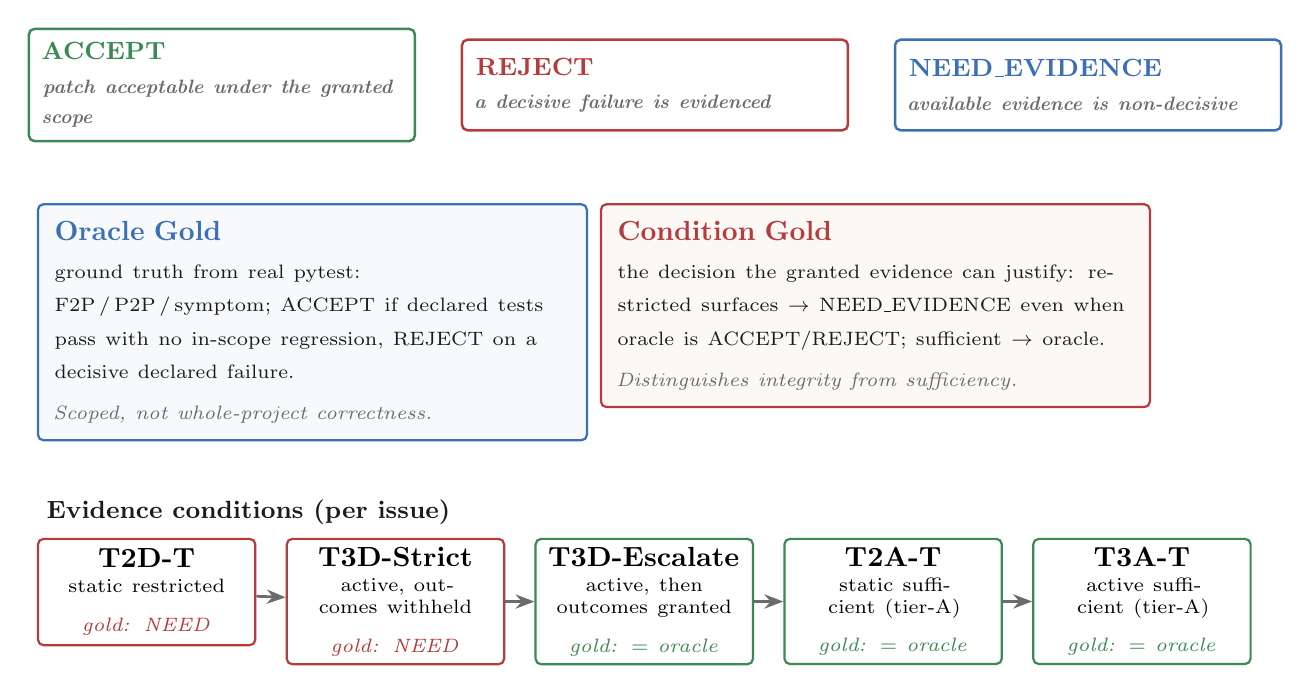
\begin{tikzpicture}[x=1cm,y=1cm,
  verdict/.style={draw,rounded corners=2pt,line width=0.9pt,align=left,
                 inner sep=5pt,text width=4.55cm,minimum height=1.15cm},
  tier/.style={draw,rounded corners=2pt,line width=0.8pt,align=left,
                 inner sep=6pt,text width=6.55cm,minimum height=2.2cm},
  cond/.style={draw,rounded corners=2pt,line width=0.8pt,align=center,
                 inner sep=3pt,text width=2.55cm,minimum height=1.35cm},
  lbl/.style={font=\scriptsize\itshape},
  >={Stealth[length=2.4mm]}]

% --- three-way verdict ---
\node[verdict,draw=grAccept,text=grAccept,font=\small\bfseries]
  (acc) at (2.35,0) {ACCEPT\\[1pt]\lbl{\textcolor{grMuted}{patch acceptable under the granted scope}}};
\node[verdict,draw=grReject,text=grReject,font=\small\bfseries]
  (rej) at (7.85,0) {REJECT\\[1pt]\lbl{\textcolor{grMuted}{a decisive failure is evidenced}}};
\node[verdict,draw=grNeed,text=grNeed,font=\small\bfseries]
  (need) at (13.35,0) {NEED\_EVIDENCE\\[1pt]\lbl{\textcolor{grMuted}{available evidence is non-decisive}}};

% --- two gold tiers ---
\node[tier,fill=grOracle,draw=grNeed,anchor=north west] (og) at (0,-1.5)
  {\textcolor{grNeed}{\bfseries Oracle Gold}\\[2pt]\normalsize
   \textcolor{grInk}{\scriptsize ground truth from real pytest: F2P\,/\,P2P\,/\,symptom;
   ACCEPT if declared tests pass with no in-scope regression, REJECT on a decisive
   declared failure.}\\[3pt]
   \lbl{\textcolor{grMuted}{Scoped, not whole-project correctness.}}};
\node[tier,fill=grCond,draw=grReject,anchor=north west] (cg) at (7.15,-1.5)
  {\textcolor{grReject}{\bfseries Condition Gold}\\[2pt]\normalsize
   \textcolor{grInk}{\scriptsize the decision the granted evidence can justify:
   restricted surfaces $\rightarrow$ NEED\_EVIDENCE even when oracle is ACCEPT/REJECT;
   sufficient $\rightarrow$ oracle.}\\[3pt]
   \lbl{\textcolor{grMuted}{Distinguishes integrity from sufficiency.}}};

% --- condition ladder label ---
\node[anchor=north west,font=\small\bfseries,text=grInk] at (0,-5.15)
  {Evidence conditions (per issue)};

% --- five condition boxes ---
\node[cond,draw=grReject,anchor=north west] (c1) at (0,-5.75)
  {\textbf{T2D-T}\\[1pt]\scriptsize static restricted\\[2pt]\textcolor{grReject}{\itshape gold: NEED}};
\node[cond,draw=grReject,anchor=north west] (c2) at (3.16,-5.75)
  {\textbf{T3D-Strict}\\[1pt]\scriptsize active, outcomes withheld\\[2pt]\textcolor{grReject}{\itshape gold: NEED}};
\node[cond,draw=grAccept,anchor=north west] (c3) at (6.32,-5.75)
  {\textbf{T3D-Escalate}\\[1pt]\scriptsize active, then outcomes granted\\[2pt]\textcolor{grAccept}{\itshape gold: $=$ oracle}};
\node[cond,draw=grAccept,anchor=north west] (c4) at (9.48,-5.75)
  {\textbf{T2A-T}\\[1pt]\scriptsize static sufficient (tier-A)\\[2pt]\textcolor{grAccept}{\itshape gold: $=$ oracle}};
\node[cond,draw=grAccept,anchor=north west] (c5) at (12.64,-5.75)
  {\textbf{T3A-T}\\[1pt]\scriptsize active sufficient (tier-A)\\[2pt]\textcolor{grAccept}{\itshape gold: $=$ oracle}};

\draw[grMuted,line width=1pt,->] (c1) -- (c2);
\draw[grMuted,line width=1pt,->] (c2) -- (c3);
\draw[grMuted,line width=1pt,->] (c3) -- (c4);
\draw[grMuted,line width=1pt,->] (c4) -- (c5);
\end{tikzpicture}

\caption{Three-way review decision, the two gold tiers, and the five-condition
evidence ladder. Restricted conditions (red) warrant \NEED; sufficient
conditions (green) warrant the Oracle Gold decision.}
\label{fig:concept}
\end{figure}

T3D-\textbf{Strict} is the key insufficiency probe: an active agent can inspect
linkage, freshness, and coverage and read the symptom, but post-patch F2P/P2P
verdicts are structurally unreachable, so accepting or rejecting necessarily
upgrades non-decisive evidence. T3D-\textbf{Escalate} grants the decisive
outcomes only after the agent explicitly requests them. The evidence-serving
protocol is summarised in Algorithm~\ref{alg:protocol}.

\begin{algorithm}[t]
\caption{GroundedReview cell protocol (one issue $i$, condition $c$, model $m$)}
\label{alg:protocol}
\begin{algorithmic}[1]
\State \textbf{input}: issue text, candidate diff, condition $c$, served model id
\State open a session bound to the candidate patch identity \Comment{no gold field is ever served}
\State $d \gets{}$ decision policy for $c$ \Comment{strict, escalate, or static}
\If{$c$ is an active (T3) condition}
  \Loop
    \State model chooses: \textsc{getArtifact}, \textsc{verifyLinkage}, \textsc{getRunLog}, or \textsc{finish}
    \If{requested field is tier-D and policy is \textsc{strict}}
       \State reply \textbf{403 forbidden} \Comment{outcomes structurally unreachable}
    \ElsIf{policy is \textsc{escalate} without a stated reason}
       \State reply \textbf{400}; require a justification
    \ElsIf{escalation justified}
       \State reply \textbf{200} with header \texttt{X-Evidence-Tier-Escalation} and the decisive outcomes
    \EndIf
  \EndLoop
\EndIf
\State persist the \textbf{raw} response before any analysis \Comment{raw-first}
\State \textbf{output}: one of \ACCEPT, \REJECT, \NEED
\State score against condition gold $\gC(i,c)$; the issue, not the cell, is the unit
\end{algorithmic}
\end{algorithm}

\paragraph{Non-interference.}
Restricted projections are machine-scanned for post-patch verdicts, hidden
gold, acceptance digests, and reconstructing keys. We disclose one residual
instrument gap found in the corrective replication: a \emph{pre-patch}
baseline P2P map survived the tier-D projection. It cannot reconstruct gold
and was seen by none of the error cells, and it is mandated for removal before
the next live run (Section~\ref{sec:threats}). The corrected v2 projection used
for the prepared validation bed removes this field on every tool path
(Section~\ref{sec:validation}).

\section{Dataset Construction}
\label{sec:dataset}

\subsection{Original ten issues (G3-A)}
Ten independently selected SymPy issue--patch pairs were used for the original
run (G3-B) and the corrective replication (G3-B.3). Oracle gold is
PROVISIONAL (single annotator). Seven are scoped \ACCEPT\ and three are
\REJECT\ (17318, 17630, 19783). The full issue list and per-issue grid are in
Appendix~\ref{app:issues}.

\subsection{Eight new independent issues (G3-C.1 pilot)}
A separate pilot constructed eight new SymPy issues, de-duplicated against
history and against each other by changed file. The selection funnel was
$75\rightarrow51\rightarrow8$: of 75 candidates, 24 mutually exclusive
exclusions (12 prior wave, 10 already in G3-A, one unavailable offline blob,
one no-clean-checkout) leave 51; a separate changed-file independence step
removes four more (distinct from the exclusion count---no double counting) to
leave 47; sampling then selects eight. Two queues of four are used:
\begin{itemize}[leftmargin=1.6em,itemsep=1pt,topsep=2pt]
  \item \textbf{Natural} (seed 418237): 19346, 22914, 19495, 15875;
  \item \textbf{REJECT-enriched} (seed 418241): 19040, 14248, 19637, 16886.
\end{itemize}
The two queues have \textbf{zero issue overlap}. Oracle distribution is six
scoped \ACCEPT\ / two \REJECT\ (14248 and 15875). Each issue has five
condition-gold certificates, giving \textbf{40 certificates: 24 sufficient, 16
\NEED}. Freshness is $8/8$; the frozen manifest lists 185 files with zero hash
mismatch.

\paragraph{Sampling disclosure.}
The enrichment category priority (TRAP $>$ P2P $>$ F2P) was an operational
refinement finalised \emph{before} any real test outcome was observed (selection
rule fixed at 09:20:33\,UTC; first pytest result at 09:48:33), but it is
\textbf{not a verbatim pre-registration}: a counterfactual F2P-first ordering
would have moved 29 strata and selected four different issues. We therefore
label it \emph{pilot-stage adaptive sampling}, not fully pre-registered, and
never pool natural and enriched queues to estimate a natural-population rate.
The two rejects arose naturally rather than being manufactured fixtures;
the independent human FR2 review rules that their distinct failure modes
instantiate one uniform disjunctive \REJECT\ standard, with no rubric
amendment required.

\subsection{Evidence-system engineering}
For the eight-issue pilot, 144 restricted surfaces return \textbf{zero}
forbidden hits; an offline HTTP cross-check retallies \textbf{456/456}
assertions; \textbf{40/40} mock cells behave as expected but are
\textbf{excluded from research analysis} (mock correctness is plumbing, not
model performance); three deterministic reruns are byte-identical. Mock and
live runs are fully isolated, and prompts and protocol are frozen and
fingerprinted before any paid call.

\section{Experimental Setup}
\label{sec:setup}

\paragraph{Models.}
Two chat models are served through a fixed client: \texttt{deepseek-flash}
(``DeepSeek'') and \texttt{gpt-4.1-mini} (``GPT''). The served model id is
asserted against the requested id; a mismatch is a hard stop, and a missing id
does not silently pass.

\paragraph{Protocol versions.}
The corrective run uses runner \texttt{g3b3-runner-v1}, protocol
\texttt{g3b2-protocol-v1}, and prompt \texttt{p3-ternary-g3b2-v1}, all frozen
and fingerprinted before the paid run. The independent-issue run uses a
separate runner \texttt{g3c1live-runner-v1} over the same frozen prompt and
the \texttt{g3c1-protocol-v1} evidence server, again fingerprinted before any
paid call. The prompt is strictly ternary:
\ACCEPT, \REJECT, or \NEED.

\paragraph{Three evidentiary classes.}
Results are kept in three classes and never pooled:
\begin{enumerate}[leftmargin=1.6em,itemsep=1pt,topsep=2pt]
  \item \textbf{Corrective replication} (G3-B.3): 100 real model cells on the
  ten original issues across both models and five conditions.
  \item \textbf{Exploratory cross-sectional analysis} (P1/P2 on G3-B.3):
  restricted-commitment and sufficient-appropriateness slices; the
  oracle-\REJECT\ slice has only three issues.
  \item \textbf{Exploratory independent-issue validation} (G3-C.1 live):
  80 real model cells on the eight \emph{disjoint}, newly constructed issues
  across both models and the same five conditions, with PROVISIONAL gold and
  \texttt{annotator2 = NOT\_OBTAINED} at run time (the independent human
  review of these packets, plus the G3-A ten, is reported in
  Section~\ref{sec:g4-human}). This is an exploratory external
  validation on a different issue set at a different time; it is not a
  human-arbitrated benchmark and is never pooled with classes 1--2.
\end{enumerate}

\paragraph{Execution accounting.}
G3-B.3 made 208 model calls (DeepSeek 114, GPT 94) at a recorded spend of
\textbf{\$0.303539} (DeepSeek \$0.189045, GPT \$0.114494) under caps of
\$3.00 total / \$1.50 per model, with zero retries, zero transport errors, and
zero resume-skips. Every response is persisted raw before analysis.

\paragraph{Independent-issue run accounting.}
The G3-C.1 live run made 162 model calls (DeepSeek 88, GPT 74) over all 80
cells at a recorded spend of \textbf{\$0.258198} (DeepSeek \$0.163936,
GPT \$0.094262; exact token-by-price arithmetic gives \$0.2581976), well
under the tightened hard caps of \$2.00 total /
\$1.00 per model. Summing the per-cell ledger entries, each rounded to six
decimals at write time, yields \$0.258199, a one-microdollar rounding
accumulation; the pre-call guard accumulator and the exact recomputation are
our reported figures. A pre-call worst-case guard bound was computed before every
paid call and enforced by both a per-model guard and one shared total guard;
retries per cell were zero, there were zero terminal errors, zero
response-format downgrades, and zero resume-skips, and every served model id
matched its asserted id. Each raw response, tool trace, token usage, cost,
served id, and parse exception was persisted before scoring.

\paragraph{Statistics.}
The unit is the issue. Where we summarise a proportion over $n$ issues we
report a Clopper--Pearson 95\,\% interval. Paired within-issue contrasts use an
issue-cluster bootstrap (10{,}000 resamples); because cells repeat within an
issue, pooled cell counts are presented with a repeated-measures caveat and are
not treated as independent. With $n\le 10$ (and $n=3$ for rejects) these
intervals are necessarily wide and are reported for honesty, not power.

\section{Results}
\label{sec:results}

All counts below are over issues and trace to the frozen result JSON
(Appendix~\ref{app:provenance}). Findings are associational; the G3-B versus
G3-B.3 contrast is cross-version (instrument and run differ), not a controlled
single-factor experiment.

\subsection{P1: Do agents respect restricted evidence?}
On the two conditions whose condition gold is \NEED\ (Table~\ref{tab:p1}),
both models abstain on every issue under the static surface T2D-T. DeepSeek
also abstains on all ten under active strict access---on $8/10$ it reached the
restricted tier-D artifact via tools and still abstained. GPT, however,
upgrades the non-decisive strict surface into \ACCEPT\ on $7/10$ issues
(13615, 13974, 15349, 17318, 17630, 21847, 24443), with only three correct
abstentions (19783, 20590, 24213). In the earlier G3-B run the same model
abstained on $10/10$; that change is a cross-version observation, not a causal
estimate of any single fix.

\begin{table}[t]
\centering
\small
\caption{P1 restricted commitment ($n=10$ issues per row; condition gold is
\NEED). ``Unsupported'' is a commit (\ACCEPT/\REJECT) where only abstention is
warranted. Pooled cell counts repeat within issue and are not independent.}
\label{tab:p1}
\begin{tabularx}{\linewidth}{@{}>{\raggedright\arraybackslash}X c c c c@{}}
\toprule
\textbf{Model -- condition} & \textbf{Unsup. \ACCEPT} & \textbf{Unsup. \REJECT} & \textbf{Correct \NEED} & \textbf{CP95 unsup.} \\
\midrule
DeepSeek -- T2D-T        & 0 & 0 & 10 & $[0.000,0.308]$ \\
DeepSeek -- T3D-Strict   & 0 & 0 & 10 & $[0.000,0.308]$ \\
GPT -- T2D-T             & 0 & 0 & 10 & $[0.000,0.308]$ \\
GPT -- T3D-Strict        & 7 & 0 & 3  & $[0.348,0.933]$ \\
\midrule
Pooled cells, DeepSeek   & \multicolumn{3}{c}{0 unsupported / 20 restricted cells} & --- \\
Pooled cells, GPT        & \multicolumn{3}{c}{7 unsupported / 20 restricted cells} & --- \\
\bottomrule
\end{tabularx}
\end{table}

\begin{figure}[t]
\centering
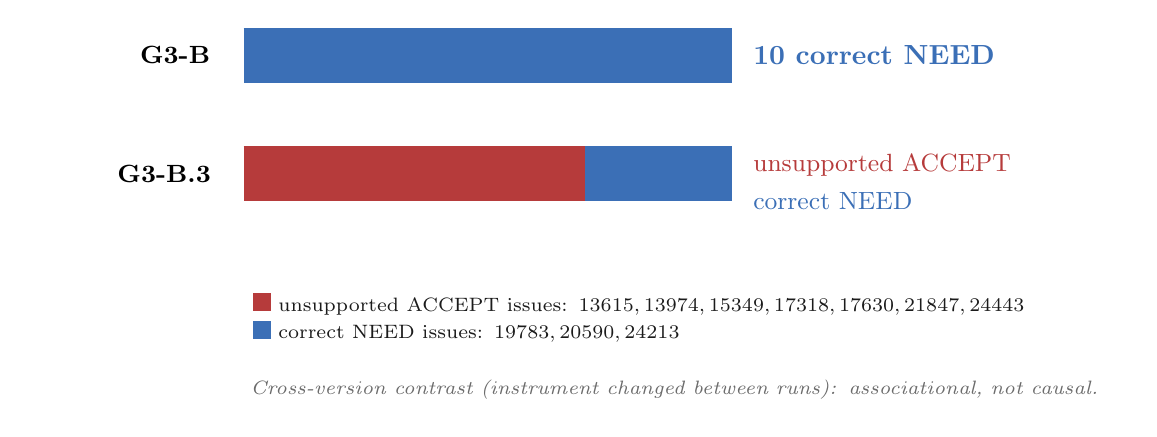
\begin{tikzpicture}[x=1cm,y=1cm,font=\small,
  >={Stealth[length=3mm]}]
\def\s{0.62}

% G3-B: 10/10 correct NEED
\node[anchor=east,text width=2.2cm,align=right] (l1) at (2.3,0.75) {\textbf{G3-B}};
\draw[line width=20pt,grNeed] (2.6,0.75) -- ($(2.6,0.75)+({10*\s},0)$);
\node[anchor=west,font=\bfseries,text=grNeed] at ($(2.6,0.75)+({10*\s+0.15},0)$) {10 correct NEED};

% G3-B.3: 7 unsupported ACCEPT + 3 correct NEED
\node[anchor=east,text width=2.2cm,align=right] (l2) at (2.3,-0.75) {\textbf{G3-B.3}};
\draw[line width=20pt,grReject] (2.6,-0.75) -- ($(2.6,-0.75)+({7*\s},0)$);
\draw[line width=20pt,grNeed] ($(2.6,-0.75)+({7*\s},0)$) -- ($(2.6,-0.75)+({10*\s},0)$);
\node[anchor=west,font=\bfseries,text=grReject] at ($(2.6,-0.75)+({7*\s/2},0)$) {7};
\node[anchor=west,font=\bfseries,text=grNeed] at ($(2.6,-0.75)+({8.5*\s},0.05)$) {3};
\node[anchor=west,text=grReject] at ($(2.6,-0.75)+({10*\s+0.15},0.1)$) {unsupported ACCEPT};
\node[anchor=west,text=grNeed] at ($(2.6,-0.75)+({10*\s+0.15},-0.35)$) {correct NEED};

% legend / issue ids
\node[anchor=north west,font=\scriptsize,text=grInk,align=left,text width=11cm] at (2.6,-2.15)
  {\textcolor{grReject}{\rule{0.8em}{0.8em}} unsupported ACCEPT issues:
   13615,\,13974,\,15349,\,17318,\,17630,\,21847,\,24443\\[2pt]
   \textcolor{grNeed}{\rule{0.8em}{0.8em}} correct NEED issues:
   19783,\,20590,\,24213};
\node[anchor=north west,font=\scriptsize\itshape,text=grMuted,align=left,text width=11cm] at (2.6,-3.25)
  {Cross-version contrast (instrument changed between runs): associational, not causal.};
\end{tikzpicture}

\caption{GPT verdicts on T3D-Strict (condition gold \NEED). G3-B (earlier
instrument) shows 10 abstentions; G3-B.3 shows seven unsupported \ACCEPT\ and
three correct \NEED. The contrast is cross-version/confounded, not causal.}
\label{fig:gptstrict}
\end{figure}

\subsection{Corrective replication: abstention under sufficient evidence}
The original G3-B run recorded DeepSeek abstaining on $9/10$ issues even when
decisive tier-A outcomes were granted. The corrective replication G3-B.3,
after repairing protocol-construct defects in our own instrument, records
$1/10$ (Figure~\ref{fig:deepseek}). Eight issues reverse from \NEED\ to a
commit, zero reverse from a commit to \NEED, and the sole residual abstention
is issue 13974.

\begin{table}[t]
\centering
\small
\caption{Correct commitment under sufficient evidence ($n=10$ per cell;
gold $=\gO$). Values are the count of issues receiving the oracle verdict.
DeepSeek: \NEED-any 9/10 in G3-B $\to$ 1/10 in G3-B.3.}
\label{tab:deepseek}
\begin{tabular}{l c c c}
\toprule
\textbf{Sufficient condition} & \textbf{G3-B} & \textbf{G3-B.3} & \textbf{CP95 (G3-B.3)} \\
\midrule
DeepSeek \NEED\textsubscript{any} & 9/10 & 1/10 & $[0.003,0.445]$ \\
\quad CP95 for G3-B $9/10$  & \multicolumn{2}{c}{$[0.555,0.997]$} & \\
\quad paired issue-cluster bootstrap of the difference & \multicolumn{2}{c}{$[0.5,1.0]$ (seed 417313)} & \\
\bottomrule
\end{tabular}
\end{table}

\begin{figure}[t]
\centering
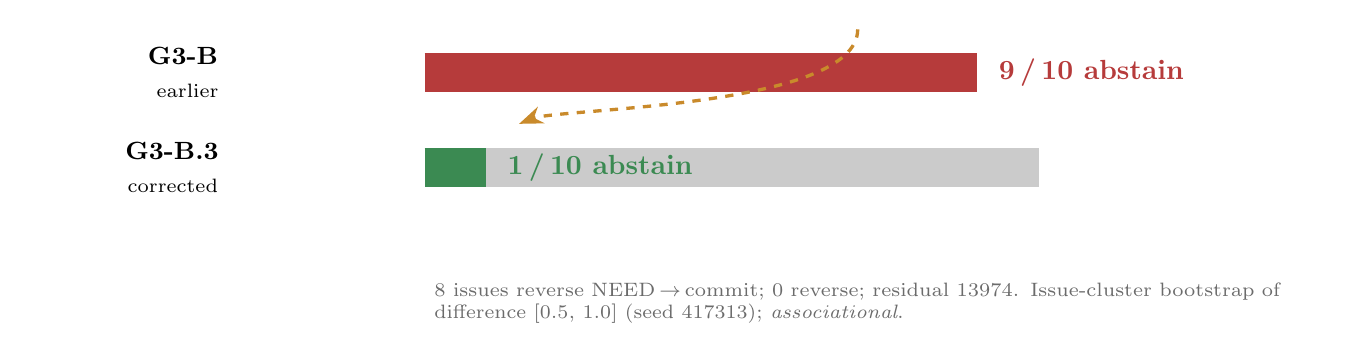
\begin{tikzpicture}[x=1cm,y=1cm,font=\small,
  barlabel/.style={anchor=east,align=right,text width=2.3cm},
  >={Stealth[length=3mm]},
  bar/.style={line width=14pt,line cap=butt}]

% scale: 1 issue = 0.78 cm ; total bar = 7.8 cm for 10
\def\s{0.78}

\node[barlabel] at (0,0.6) {\textbf{G3-B}\\[1pt]\scriptsize earlier};
\draw[bar,grReject] (2.5,0.6) -- ($(2.5,0.6)+({9*\s},0)$);
\node[anchor=west,text=grReject,font=\bfseries] at ($(2.5,0.6)+({9*\s+0.15},0)$) {9\,/\,10 abstain};

\node[barlabel] at (0,-0.6) {\textbf{G3-B.3}\\[1pt]\scriptsize corrected};
\draw[bar,grAccept] (2.5,-0.6) -- ($(2.5,-0.6)+({1*\s},0)$);
\draw[bar,grMuted!35] ($(2.5,-0.6)+({1*\s},0)$) -- ($(2.5,-0.6)+({10*\s},0)$);
\node[anchor=west,text=grAccept,font=\bfseries] at ($(2.5,-0.6)+({1*\s+0.15},0)$) {1\,/\,10 abstain};

% dashed transition arrow
\draw[grWarn,dashed,line width=1.2pt,->] (8.0,1.15) .. controls (8.0,0.15) and (4.2,0.15) .. (3.7,-0.05);
\node[font=\scriptsize,text=grMuted,align=left,anchor=north west,text width=11.2cm] at (2.5,-1.95)
  {8 issues reverse NEED\,$\to$\,commit; 0 reverse; residual 13974.
   Issue-cluster bootstrap of difference $[0.5,\,1.0]$ (seed 417313); \textit{associational}.};
\end{tikzpicture}

\caption{DeepSeek sufficient-evidence abstention, $9/10 \to 1/10$ after the
instrument was repaired. Eight issues reverse to a commit; the residual is
13974. Associational cross-version contrast; issue-cluster bootstrap
$[0.5,1.0]$.}
\label{fig:deepseek}
\end{figure}

\subsection{Sufficient-evidence appropriateness}
Table~\ref{tab:p2main} reports oracle-consistent verdicts on the three
sufficient conditions. DeepSeek is correct on $9/10$ under T3D-Escalate and
T2A-T and $10/10$ under active T3A-T. GPT is correct on $8/10$ under escalate
and static sufficient access (one wrong \ACCEPT\ on reject issue 17318 and one
over-abstention on 17630) and $9/10$ under T3A-T, where active access flips
17318 to a correct \REJECT\ while 17630 remains an abstention.

\begin{table}[t]
\centering
\small
\caption{Sufficient-evidence appropriateness: oracle-consistent verdicts out
of 10 issues per condition.}
\label{tab:p2main}
\begin{tabular}{l c c c}
\toprule
\textbf{Condition} & \textbf{DeepSeek} & \textbf{GPT} & \textbf{GPT residual errors} \\
\midrule
T3D-Escalate & 9/10 & 8/10 & 1 wrong \ACCEPT\ (17318); 1 abstain (17630) \\
T2A-T        & 9/10 & 8/10 & 1 wrong \ACCEPT\ (17318); 1 abstain (17630) \\
T3A-T        & 10/10 & 9/10 & 1 abstain (17630); 17318 flips to correct \REJECT \\
\bottomrule
\end{tabular}
\end{table}

\subsection{P2 exploratory slice on the three oracle-REJECT issues}
For the three oracle-\REJECT\ issues (17318, 17630, 19783), GPT returns an
unsupported \ACCEPT\ in $4/15$ sufficient cells. Aggregating to the issue
level (correct rejection under \emph{any} sufficient condition), GPT correctly
rejects $2/3$ issues, CP95 $[0.094,0.992]$; the issue-cluster bootstrap spans
$[0,1]$ (seed 313). With three rejects we report \textbf{no rate}: this is an
exploratory slice only, and the new pilot adds only two more rejects, so it
remains exploratory even after a live run.

\subsection{Exploratory validation on eight independent issues (G3-C.1 live)}
\label{sec:e80}
We ran the same two models and five frozen conditions on a \emph{disjoint}
set of eight newly constructed issues (six oracle-\ACCEPT, two
oracle-\REJECT): 80 real cells, 162 model calls, spend \$0.258 under
\$2.00/\$1.00 hard caps, zero retries or errors. Gold is PROVISIONAL and
this is a different issue set at a different time, so every comparison below
is an associational cross-set observation, never a causal estimate, and the
slice is not pooled with Sections~\ref{sec:results}--7.3.

On the two restricted conditions (condition gold \NEED), DeepSeek abstains on
all $8/8$ issues under \emph{both} T2D-T and active T3D-Strict. GPT abstains
on all $8/8$ under the static T2D-T surface but, under active strict access,
again upgrades the non-decisive surface to unsupported \ACCEPT\ on $6/8$
issues (CP95 $[0.349,0.968]$); the two correct abstentions are 19637 and
16886. Notably the six unsupported strict \ACCEPT\ verdicts include
\emph{both} oracle-\REJECT\ issues (14248, 15875): under restricted
diagnostic-only evidence the model committed ``accept'' on patches that
fresh, scoped, sufficient evidence adjudicates as failing. The recurring
GPT strict-over-commitment on a second, independent issue set
($7/10 \to 6/8$) is the central cross-set replication; the instruments,
issue sets, and run times differ, so we do not attribute the recurrence to a
single cause.

\begin{table}[t]
\centering
\small
\caption{P1 restricted commitment on the eight independent issues (condition
gold \NEED). ``Unsupported'' is a commit where abstention is warranted.
Issue-level CP95 (Clopper--Pearson); pooled cells are repeated measures.}
\label{tab:p1e80}
\begin{tabularx}{\linewidth}{@{}>{\raggedright\arraybackslash}X c c c c@{}}
\toprule
\textbf{Model -- condition} & \textbf{Unsup. \ACCEPT} & \textbf{Unsup. \REJECT} & \textbf{Correct \NEED} & \textbf{CP95 unsup.} \\
\midrule
DeepSeek -- T2D-T        & 0 & 0 & 8 & $[0.000,0.369]$ \\
DeepSeek -- T3D-Strict   & 0 & 0 & 8 & $[0.000,0.369]$ \\
GPT -- T2D-T             & 0 & 0 & 8 & $[0.000,0.369]$ \\
GPT -- T3D-Strict        & 6 & 0 & 2 & $[0.349,0.968]$ \\
\midrule
Pooled cells, DeepSeek   & \multicolumn{3}{c}{0 unsupported / 16 restricted cells} & --- \\
Pooled cells, GPT        & \multicolumn{3}{c}{6 unsupported / 16 restricted cells} & --- \\
\bottomrule
\end{tabularx}
\end{table}

\begin{table}[t]
\centering
\small
\caption{Ternary verdict matrix for the 80-cell independent-issue run:
counts of \ACCEPT/\REJECT/\NEED\ out of 8 issues per model--condition.
Restricted rows (top two) have condition gold \NEED; sufficient rows
(bottom three) have gold $=$ oracle (6 \ACCEPT, 2 \REJECT).}
\label{tab:matrixe80}
\begin{tabular}{l c ccc ccc}
\toprule
 & & \multicolumn{3}{c}{\textbf{DeepSeek}} & \multicolumn{3}{c}{\textbf{GPT}} \\
\cmidrule(lr){3-5}\cmidrule(lr){6-8}
\textbf{Condition} & \textbf{Class} & A & R & N & A & R & N \\
\midrule
T2D-T        & restricted & 0 & 0 & 8 & 0 & 0 & 8 \\
T3D-Strict   & restricted & 0 & 0 & 8 & 6 & 0 & 2 \\
T3D-Escalate & sufficient & 6 & 2 & 0 & 6 & 1 & 1 \\
T2A-T        & sufficient & 5 & 2 & 1 & 6 & 2 & 0 \\
T3A-T        & sufficient & 6 & 2 & 0 & 6 & 2 & 0 \\
\bottomrule
\end{tabular}
\end{table}

Under sufficient evidence both models reach the oracle verdict on $8/8$
issues at active tier-A (T3A-T): six \ACCEPT\ and two correct \REJECT. On the
other sufficient conditions coverage is $7/8$--$8/8$: DeepSeek is $8/8$ under
T3D-Escalate and $7/8$ under T2A-T (one over-abstention on \ACCEPT\ issue
19495); GPT is $7/8$ under T3D-Escalate (one over-abstention on \REJECT\
issue 15875) and $8/8$ under T2A-T. Neither model returns an unsupported
\ACCEPT\ on either \REJECT\ issue once sufficient evidence is granted.

\paragraph{P2 exploratory reject slice ($n=2$).}
Aggregating to the issue level (an issue is flagged only if \emph{no}
sufficient condition yields a correct \REJECT), both models correctly reject
both \REJECT\ issues (14248, 15875): unsupported-\ACCEPT\ rate $0/2$, CP95
$[0.000,0.842]$, issue-cluster bootstrap $[0,0]$ (seed 418388,
$B=10{,}000$). With only two \REJECT\ issues this is a pair of cases with an
interval, \emph{not} a population error rate; we draw no rate conclusion.

\subsection{Case studies}
\label{sec:cases}
\paragraph{F1 --- Issue 17318, ignored visible failure.}
On the static sufficient surface T2A-T the declared fail-to-pass test
\texttt{test\_issue\_12420} is already present and visibly \textbf{FAILED} with
\texttt{assert [4 + I, 0, 1] == []}; GPT nevertheless returns \ACCEPT, in both
G3-B and G3-B.3. On the active sufficient surface T3A-T it reaches the failure
and correctly returns \REJECT\ (Figure~\ref{fig:focal}). This is an $n=3$
qualitative case, not a rate: the same decisive artifact is accepted when
statically presented and rejected when actively fetched.

\begin{figure}[t]
\centering
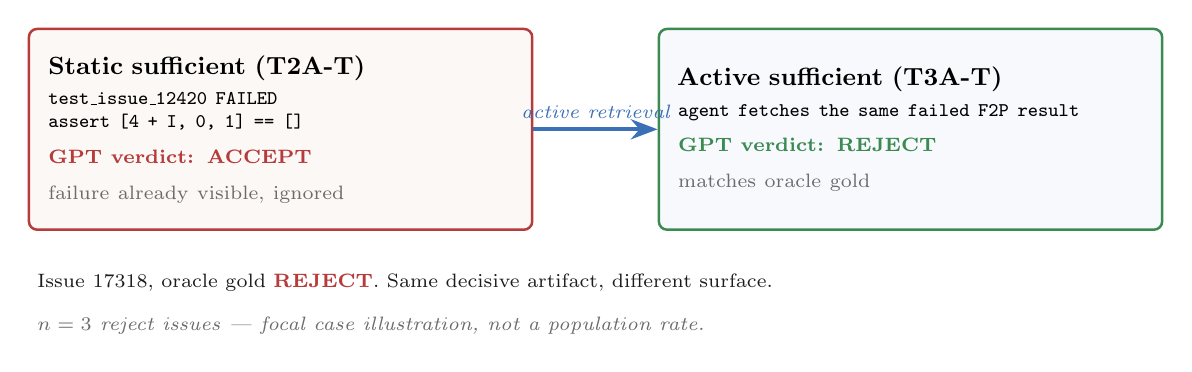
\begin{tikzpicture}[x=1cm,y=1cm,font=\small,
  panel/.style={draw,rounded corners=3pt,line width=0.9pt,align=left,
                inner sep=7pt,text width=5.9cm,minimum height=2.55cm},
  >={Stealth[length=3.4mm]}]

\node[panel,fill=grCond,draw=grReject,anchor=north west] (p1) at (0,0)
  {\textbf{Static sufficient (T2A-T)}\\[3pt]\ttfamily\scriptsize
   test\_issue\_12420 \textbf{FAILED}\\
   assert [4 + I, 0, 1] == []\\[5pt]\rmfamily
   \textcolor{grReject}{\bfseries GPT verdict: ACCEPT}\\[2pt]
   \scriptsize\textcolor{grMuted}{failure already visible, ignored}};

\node[panel,fill=grOracle,draw=grAccept,anchor=north west] (p2) at (8.0,0)
  {\textbf{Active sufficient (T3A-T)}\\[3pt]\ttfamily\scriptsize
   agent fetches the same failed F2P result\\[5pt]\rmfamily
   \textcolor{grAccept}{\bfseries GPT verdict: REJECT}\\[2pt]
   \scriptsize\textcolor{grMuted}{matches oracle gold}};

\draw[line width=1.4pt,grNeed,->] (p1.east) -- node[above,font=\scriptsize\itshape,text=grNeed]{active retrieval} (p2.west);

\node[anchor=north west,font=\scriptsize,text=grInk] at (0,-3.0)
  {Issue 17318, oracle gold \textcolor{grReject}{\bfseries REJECT}. Same decisive artifact, different surface.};
\node[anchor=north west,font=\scriptsize\itshape,text=grMuted] at (0,-3.55)
  {$n=3$ reject issues --- focal case illustration, not a population rate.};
\end{tikzpicture}

\caption{Focal case 17318 (oracle \REJECT). A statically presented, already
failed F2P test is ignored (\ACCEPT); active retrieval of the same failure
yields \REJECT. Case evidence, not a population rate.}
\label{fig:focal}
\end{figure}

\paragraph{F2 --- Issue 17630, over-abstention.}
On T3A-T the model observes a failed \path{test_zero_matrix_add}, judges
it unrelated to the patch, and returns \NEED\ rather than committing. This is
the residual abstention under otherwise decisive access and illustrates the
opposite failure mode from F1: under-use rather than over-use of evidence.

\paragraph{Residual DeepSeek abstention --- 13974.}
DeepSeek's single residual abstention rests on a belief that
\texttt{test\_tensor\_product\_simp} is missing; the test is in fact present
and passing (it is added by the patch itself), and the compared logs are not
identical, so the abstention is not well grounded even under the agent's own
reasoning.

\paragraph{Qualitative coding.}
A single AI-assisted coding pass (coder masked as D01--D07) over the seven
GPT strict accepts attributes each to the code \textbf{C3}: treating
\emph{absence of failure evidence as evidence of absence}. A hypothesised
second mechanism (C4) never fires and is therefore reported only as a
qualitative hypothesis, not a counted category.

\section{Ablations and Instrument Findings}
\label{sec:ablations}

\subsection{Static vs.\ active restricted access}
\label{sec:mechanism}
All unsupported commitments arise on the \emph{active} strict condition; the
static restricted condition is $10/10$ correct for both models. A partially
blind coding of GPT's seven strict accepts (codebook frozen before coding;
packets masked D01--D07) assigns the primary code \textbf{C3}---treating
\emph{absence of failure evidence as evidence of absence}---to all seven,
co-firing C1 (symptom resolution), C2 (coverage completeness), and C5
(provenance/freshness); \textbf{C4} (explicitly acknowledging the withholding)
never fires. This is a \emph{single AI rule-based coder with no independent
human coder}, so it is a qualitative hypothesis only. Moreover activeness,
freshness, and trust changed together across protocol versions, so the
active/static comparison is confounded; an activeness-only controlled arm
(freshness and trust held fixed) is required before calling this a demonstrated
mechanism.

\subsection{Instrument residual: baseline P2P projection gap}
The tier-1 non-interference scan was $61/61$ clean, but a tier-2 minimisation
found the \emph{pre-patch} \texttt{pass\_to\_pass\_baseline} per-test map
surviving the tier-D projection (all \textsc{Pass}, zero \textsc{Fail}). It
cannot reconstruct gold (the post-patch P2P map is removed), was reachable only
by explicit fetch, and was seen by none of the seven error cells: the single GPT
cell that saw it (20590) abstained, and DeepSeek saw it in eight cells and
abstained throughout. It therefore has no causal link to the reported errors,
but it is a disclosed non-interference imperfection and is mandated for removal
before the next live run. The corrected v2 projection used for the prepared
80-cell validation bed removes this field on every tool path
(Section~\ref{sec:validation}).

\subsection{Independent-issue pilot status}
The eight G3-C.1 issues rest on 40 gold certificates, evidence projections
with $144/144$ clean restricted surfaces (224 surfaces total), $456/456$ HTTP
cross-checks, and frozen manifests. This measurement bed was subsequently
exercised by the live 80-cell run (Section~\ref{sec:e80}). Mock cells used
during engineering contribute \emph{zero} model-performance datapoints, are
not used to fill any results cell, and are excluded from research analysis;
every reported datapoint comes from a real, raw-first-persisted model
response.

\subsection{External validation: engineering readiness and live execution}
\label{sec:validation}
An 80-cell external validation on the eight new issues (2 models $\times$
5 conditions $\times$ 8 issues) was engineered, cleared every offline gate at
\$0, received separate written authorization, and then ran to completion
(Section~\ref{sec:e80}). Pre-paid readiness checks reported:
\begin{itemize}[leftmargin=1.6em,itemsep=1pt,topsep=2pt]
  \item \textbf{non-interference:} 224 surfaces probed; 144 restricted
  tier-D; \textbf{0} tier-1, \textbf{0} tier-2, \textbf{0} baseline, and
  \textbf{0} hidden-gold exposures; $40/40$ dedicated mock gold alignments
  ($64/64$ non-Escalate cells through the generic script);
  \item \textbf{protocol:} strict 403 on all 8 restricted fetches; escalation
  400-without-reason then 200-with-reason on all 8; v2 projection tag present;
  \item \textbf{model id:} exact served-id match, hard stop on drift, no false
  trip when id absent;
  \item \textbf{budget/resume/raw-first:} guards at \$2.00 total / \$1.00 per
  model (allow + per-cell cap + per-model block + total block, both models);
  resume restores accumulated spend and refuses NaN/Inf/negative ledgers;
  raw-first persistence sha-verified on all 80 raw artifacts before scoring.
\end{itemize}
The pre-run engineering verdict was \texttt{ENGINEERING\_READY}, with three
\emph{non-engineering} items tracked in
\path{paper_sprint/experiment80/READINESS.md}: (i)~\textbf{authorization}
for live model calls, since granted in writing for 80 cells at the
\$2.00/\$1.00 caps; (ii)~\textbf{gold authority}---\texttt{annotator2 =
NOT\_OBTAINED}, so the run is reported as a \emph{Provisional-Gold Exploratory
Evaluation}, not human-arbitrated benchmark validation (PROVISIONAL by
design); and (iii)~\textbf{runner binding}---a dedicated live runner
(\texttt{g3c1live-runner-v1}), instantiated for the eight G3-C.1 issues at
\$2.00/\$1.00 and fingerprinted pre-run, rather than the frozen G3-B.3
entrypoint (which defaults to \$3.00/\$1.50 and the G3-A store). The bound
runner completed $80/80$ cells, 162 calls, spend \$0.258198, with zero
retries, terminal errors, response-format downgrades, and resume-skips.

\subsection{From instrument findings to a controlled intervention}
The mechanism codes above (notably C2/C5: completeness and provenance acting
as acceptance warrants despite withheld decisive results) are associational
and rely on partially blind qualitative coding. G4
(Section~\ref{sec:g4}) tests that mechanism causally: linkage is fixed, the
evidence transcript is yoked, and only decisive-outcome visibility and
freshness/coverage attestation vary. The G4 H1 result supplies the
controlled counterpart to the C5-style explanation suggested here.

\section{G4: A Controlled Intervention on Sufficiency vs.\ Attestation}
\label{sec:g4}

Sections~\ref{sec:results}--\ref{sec:e80} are associational: instrument,
issue set, and run time co-vary. G4 is a \emph{controlled intervention} that
holds linkage constant and randomises, within the same 18 frozen issue--patch
pairs, exactly two factors in a $2\times2$ design, so that a paired contrast
identifies a causal effect under the frozen protocol.

\subsection{Design, factors, and identification}
\label{sec:g4-design}
Each issue is served under four cells defined by two binary factors.
Factor $O$ is \emph{decisive-outcome visibility}: whether the fail-to-pass
and scoped pass-to-pass test verdicts are blocked (\texttt{403 STRICT\_403})
or visible (real post-patch logs with status 200). Factor $M$ is
\emph{freshness/coverage attestation}: whether the independently recomputed
freshness and coverage certificates are withheld (nulls plus an explicit
\texttt{UNKNOWN} marker) or shown adjudicated. \textbf{Linkage is held
constant} across all four cells: artifact signing, \texttt{patch\_sha256},
and \texttt{base\_commit} linkage are identical everywhere (see
Table~\ref{tab:g4-cells}). We deliberately do not fabricate stale or
incomplete evidence: neutralised freshness/coverage cannot be reconstructed
authentically, so $M$ manipulates attestation \emph{visibility} while the
underlying facts are all TRUE, and the experiment identifies the effect of
\emph{attestation under blocked decisive outcomes}, not of genuine evidence
corruption.

\begin{table}[t]
\centering\small
\caption{G4 $2\times2$ cells. $O$ = decisive F/C verdict visibility;
$M$ = freshness/coverage attestation; linkage is constant across all cells.
Condition gold is \NEED\ in A/B (decisive outcomes withheld); in C/D it
equals oracle gold.}
\label{tab:g4-cells}
\begin{tabular}{c c c l}
\toprule
\textbf{Cell} & \textbf{$O$ decisive results} & \textbf{$M$ attestation} & \textbf{Condition gold} \\
\midrule
A & blocked & withheld       & \NEED\ (all 18) \\
B & blocked & adjudicated    & \NEED\ (all 18) \\
C & visible & withheld       & $=$ oracle \\
D & visible & adjudicated    & $=$ oracle \\
\bottomrule
\end{tabular}
\end{table}

The same frozen nine-step evidence transcript (artifact, linkage, freshness,
coverage, consistency, symptom probe, then F2P/P2P/baseline results) is
replayed to the model in a fixed order: the agent never selects a tool path,
and tool calls are yoked rather than generated. Every cell runs in an
independent context (20 messages: system, user, nine scripted tool calls and
nine tool results) followed by exactly one paid decision call
(temperature~0, bounded length, strict JSON schema, no tools exposed on the
final call). The 144 slots (18 issues $\times$ 4 cells $\times$ 2 models)
were executed once each in a frozen paired Latin order
(seed \texttt{20261102}), balanced to eight slots per issue block; a
successful cell was never re-sampled. The primary, two-sided, pre-registered
test is H1: unsupported acceptance under A versus B, an issue-paired exact
McNemar test, with the paired difference and an issue-clustered bootstrap
95\,\% interval. C/D are \emph{diagnostic controls}, not a pass/fail arm.
The frozen issue set is 13 oracle-\ACCEPT\ and 5 oracle-\REJECT; all gold
remain PROVISIONAL as primary scoring labels, although an independent human
second annotation has since been obtained
(Section~\ref{sec:g4-human}).

\subsection{H1 primary result: attestation under blocked decisive outcomes}
\label{sec:g4-h1}
Table~\ref{tab:g4-verdicts} reports the full ternary matrix; there were zero
invalid or unparseable outputs and zero response-format downgrades in 144
cells. Under cell~A every verdict from both models is \NEED: with neither
decisive results nor freshness/coverage attestation visible, neither model
commits. Under cell~B the models diverge sharply.

\begin{table}[t]
\centering\small
\caption{G4 ternary verdict matrix, counts out of 18 issues per model--cell.
Condition gold: \NEED\ for A/B; oracle (13 \ACCEPT, 5 \REJECT) for C/D.}
\label{tab:g4-verdicts}
\begin{tabular}{l c c c c}
\toprule
\textbf{Model -- cell} & \textbf{\ACCEPT} & \textbf{\REJECT} & \textbf{\NEED} & \textbf{Invalid} \\
\midrule
GPT -- A   & 0  & 0 & 18 & 0 \\
GPT -- B   & 8  & 0 & 10 & 0 \\
GPT -- C   & 13 & 4 & 1  & 0 \\
GPT -- D   & 12 & 5 & 1  & 0 \\
\midrule
DeepSeek -- A & 0  & 0 & 18 & 0 \\
DeepSeek -- B & 0  & 0 & 18 & 0 \\
DeepSeek -- C & 12 & 6 & 0  & 0 \\
DeepSeek -- D & 12 & 6 & 0  & 0 \\
\bottomrule
\end{tabular}
\end{table}

\begin{table}[t]
\centering\small
\caption{H1 pre-registered primary test, A vs.\ B unsupported acceptance
($n=18$ paired issues per model). $b$: unsupported only in A; $c$:
unsupported only in B; two-sided exact (binomial) McNemar; interval is an
issue-clustered nonparametric bootstrap ($B=20{,}000$, seed 20261102).
Models are reported separately and are never pooled.}
\label{tab:g4-h1}
\begin{tabular}{l c c c c c c}
\toprule
\textbf{Model} & \textbf{$U(A)$} & \textbf{$U(B)$} & \textbf{$b$} & \textbf{$c$} & \textbf{$p$ (two-sided)} & \textbf{$\hat\Delta_{A-B}$ [95\% CI]} \\
\midrule
GPT-4.1-mini     & 0/18 & 8/18 & 0 & 8 & 0.0078 & $-0.444$ [$-0.667,-0.222$] \\
DeepSeek-Flash   & 0/18 & 0/18 & 0 & 0 & 1.0000 & $0.000$ [$0.000,0.000$] \\
\bottomrule
\end{tabular}
\end{table}

For GPT-4.1-mini, adding adjudicated freshness/coverage attestation while
\emph{keeping the decisive test verdicts blocked} moves 8 of 18 issues from
\NEED\ to unsupported \ACCEPT, with zero moves in the opposite direction
(Table~\ref{tab:g4-h1}, Figure~\ref{fig:g4gpt}). The paired, two-sided exact
McNemar test gives $p=0.0078$; the paired difference is $-0.444$ with
issue-clustered 95\,\% bootstrap interval $[-0.667,-0.222]$, which excludes
zero. The pre-registered exact Clopper--Pearson interval for the B-cell
unsupported-acceptance rate $8/18$ is $[0.215,0.692]$ (the corresponding
interval for every $0/18$ cell is $[0,0.185]$). Under the frozen yoked
protocol this identifies a causal effect of attestation visibility: integrity
certificates that say nothing about sufficiency are sufficient for this model
to upgrade a non-decisive surface into acceptance. The eight issues include
both kinds of oracle: two of the five oracle-\REJECT\ patches (14248, 15875)
and six of the thirteen oracle-\ACCEPT\ patches (16886, 19495, 22914, 13615,
13974, 15349).

DeepSeek-Flash shows no movement at all: 18/18 \NEED\ in both A and B, zero
discordant pairs, $p=1.0$ (Figure~\ref{fig:g4deepseek}). The intervention
does not move this model, and we report the null plainly rather than pooling
the two models. The contrast is model heterogeneity, not a universal
mechanism: GPT treats adjudicated integrity as a warrant to accept despite
withheld decisive results, whereas DeepSeek keeps gating on the decisive
verdicts themselves. We cannot distinguish, from this design, whether
DeepSeek's abstention reflects well-calibrated sufficiency judgment or a
blanket conservative policy, and the zero variance in A/B also makes its
estimate degenerate.

\begin{figure}[t]
\centering
% G4 paired A->B unsupported-acceptance transitions, GPT-4.1-mini (n=18)
% n11=0  b(A only)=0  c(B only)=8  n00=10 ; exact two-sided McNemar p=0.0078
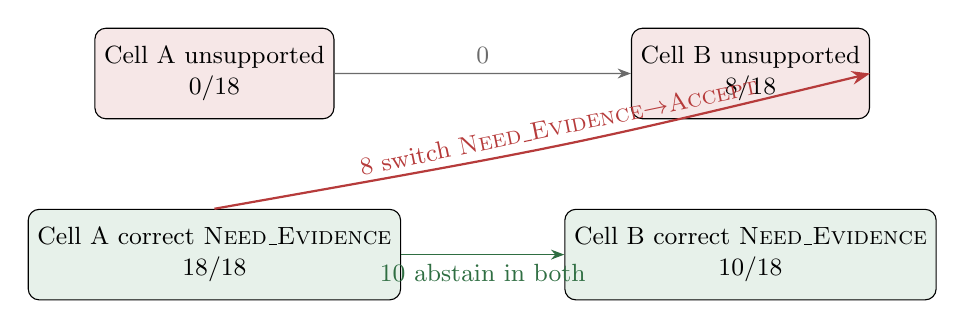
\begin{tikzpicture}[scale=0.92, every node/.style={font=\small},
  box/.style={draw,rounded corners,minimum width=2.9cm,minimum height=1.15cm,align=center}]
  \node[box,fill=grReject!12] (a1) at (0,2.5)
    {Cell A unsupported\\$0/18$};
  \node[box,fill=grAccept!12] (a0) at (0,0)
    {Cell A correct \NEED\\$18/18$};
  \node[box,fill=grReject!12] (b1) at (7.4,2.5)
    {Cell B unsupported\\$8/18$};
  \node[box,fill=grAccept!12] (b0) at (7.4,0)
    {Cell B correct \NEED\\$10/18$};
  \draw[-Stealth,grMuted] (a1) -- (b1) node[midway,above]{$0$};
  \draw[-Stealth,grReject,thick] (a0.north) .. controls (4.9,1.5) .. (b1.east)
    node[midway,above,sloped]{$8$ switch \NEED$\to$\ACCEPT};
  \draw[-Stealth,grAccept!80!black] (a0) -- (b0) node[midway,below]{$10$ abstain in both};
\end{tikzpicture}

\caption{G4 paired A$\to$B transitions for GPT-4.1-mini ($n=18$). Eight
issues switch from correct \NEED\ in A to unsupported \ACCEPT\ in B; none
switch back; ten abstain in both. Two-sided exact McNemar $p=0.0078$.}
\label{fig:g4gpt}
\end{figure}

\begin{figure}[t]
\centering
% G4 paired A->B unsupported-acceptance transitions, DeepSeek-Flash (n=18)
% n11=0  b=0  c=0  n00=18 ; exact two-sided McNemar p=1.0 (null)
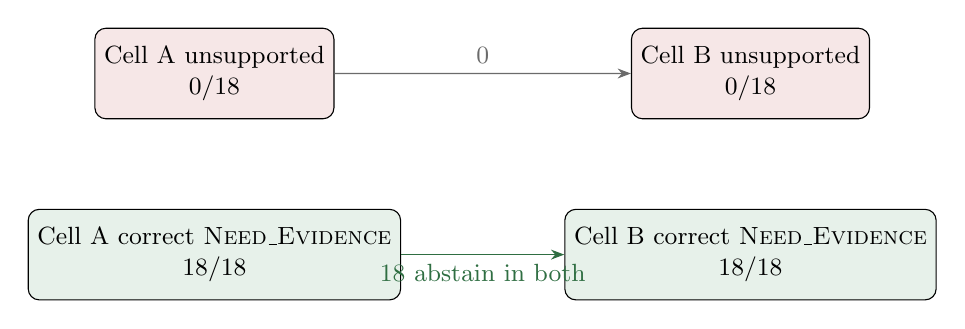
\begin{tikzpicture}[scale=0.92, every node/.style={font=\small},
  box/.style={draw,rounded corners,minimum width=2.9cm,minimum height=1.15cm,align=center}]
  \node[box,fill=grReject!12] (a1) at (0,2.5)
    {Cell A unsupported\\$0/18$};
  \node[box,fill=grAccept!12] (a0) at (0,0)
    {Cell A correct \NEED\\$18/18$};
  \node[box,fill=grReject!12] (b1) at (7.4,2.5)
    {Cell B unsupported\\$0/18$};
  \node[box,fill=grAccept!12] (b0) at (7.4,0)
    {Cell B correct \NEED\\$18/18$};
  \draw[-Stealth,grMuted] (a1) -- (b1) node[midway,above]{$0$};
  \draw[-Stealth,grAccept!80!black] (a0) -- (b0) node[midway,below]{$18$ abstain in both};
\end{tikzpicture}

\caption{G4 paired A$\to$B transitions for DeepSeek-Flash ($n=18$). All 18
issues abstain in both cells; there are no discordant pairs (exact
$p=1.0$). Reported as a null for this model.}
\label{fig:g4deepseek}
\end{figure}

\subsection{C/D diagnostic controls: what decisive visibility adds}
\label{sec:g4-cd}
When the decisive F/C results are visible, unsupported acceptance on the
five oracle-\REJECT\ issues is $0/5$ for both models under both C and D, and
oracle agreement over all 18 issues is high: GPT matches the oracle on
17/18 (C) and 16/18 (D); DeepSeek on 17/18 in both (Table~\ref{tab:g4-cd}).
Visibility of the decisive verdicts, not attestation, is what lets both
models reject the failing patches. Within C versus D, DeepSeek is identical
(12 \ACCEPT, 6 \REJECT) and GPT differs on a single issue (13 vs.\ 12
\ACCEPT): the $M$ attestation factor has essentially no additional effect
once $O$ is visible (diagnostic exact McNemar on the five rejects is
degenerate, $p=1.0$). The residual non-oracle verdicts are concentrated on
two issues. DeepSeek returns \REJECT\ on oracle-\ACCEPT\ issue~19346 under
both C and D; GPT returns \REJECT\ on 19346 only under D and accepts it under
C, and GPT additionally over-abstains (\NEED) on oracle-\REJECT\ issue~17630
under both C and D. Issue~19346 is the packet with the pre-existing
GLM-vs-provisional-oracle disagreement and has its own independent human
arbitration worksheet; it is distinct from focused review FR1 (the 19495
probe-revision question, Section~\ref{sec:threats}). These are treated as
diagnostic observations, not as failures of the primary test. The human
review of these packets has now returned (Section~\ref{sec:g4-human}):
FR1 and FR2 are closed and the 19346 arbiter records \REJECT.

\begin{table}[t]
\centering\small
\caption{C/D diagnostic control. Oracle agreement out of 18; unsupported
\ACCEPT\ on the five oracle-\REJECT\ issues out of 5; ternary counts shown
for context. C/D are diagnostic, not a pass/fail arm.}
\label{tab:g4-cd}
\begin{tabular}{l c c c c}
\toprule
\textbf{Model} & \textbf{Oracle match C / D} & \textbf{$U$ on 5 rejects C / D} & \textbf{C (A/R/N)} & \textbf{D (A/R/N)} \\
\midrule
GPT-4.1-mini   & 17/18 / 16/18 & 0/5 / 0/5 & 13/4/1 & 12/5/1 \\
DeepSeek-Flash & 17/18 / 17/18 & 0/5 / 0/5 & 12/6/0 & 12/6/0 \\
\bottomrule
\end{tabular}
\end{table}

\subsection{Strata, sensitivity, and interaction}
\label{sec:g4-sens}
Table~\ref{tab:g4-strata} splits H1 by oracle. The GPT B-cell over-acceptance
occurs on $6/13$ oracle-\ACCEPT\ and $2/5$ oracle-\REJECT\ issues; exact
Clopper--Pearson 95\,\% intervals are $[0.192,0.749]$ and $[0.053,0.853]$,
respectively, so the REJECT-stratum estimate is reported as a small-sample
observation, not a rate. Every A-cell count is zero in both strata for both
models.
%
Sensitivity analyses: (i)~the pre-registered parser rule treats unparseable
output as non-acceptance; there were zero parse failures, so the complete-case
analysis is identical to the primary analysis; (ii)~flipping the five
provisional \REJECT\ labels to \ACCEPT\ would remove all C/D unsupported
accepts by construction, while flipping all 13 \ACCEPT\ labels to \REJECT\
would make every C/D \ACCEPT\ unsupported (GPT 13/12, DeepSeek 12/12)---the
primary A/B endpoint, whose condition gold is \NEED\ independent of oracle
gold, is unchanged by either flip; (iii)~the model contrast is strictly
\emph{exploratory}: on the same 18 issues paired across models, the A/B
intervention effect differs between models by $0.444$ with an issue-paired
bootstrap 95\,\% interval $[0.222,0.667]$, and a four-cell
difference-in-differences on the only endpoint defined identically in all
four cells---raw binary acceptance $Y=\mathbf{1}\{\ACCEPT\}$, not $U$, whose
scoring rule changes across $O$---gives $\mathrm{DiD}_{\mathrm{GPT}}=0.500$
(GPT: $(8-0)/18-(12-13)/18$), $\mathrm{DiD}_{\mathrm{DS}}=0$ (identical C and
D: $12/18$), and interaction $\mathrm{DiD}_{\mathrm{GPT}}-\mathrm{DiD}_{
\mathrm{DS}}=0.500$, bootstrap 95\,\% $[0.278,0.722]$. Neither model contrast
was pre-registered as confirmatory, there is no multiplicity adjustment, and
with 18 issues (5 rejects) we make no causal claim beyond the within-model
paired H1 identifications. (An earlier internal draft labelled $-1/18$ vs.\
$0$, the between-model difference of the visible-cell contrast
$\overline{Y_D-Y_C}$, as a ``difference-in-differences of 0.056''; that number
is a simple $O$-visibility contrast, not an interaction.)

\begin{table}[t]
\centering\small
\caption{Unsupported acceptance by oracle stratum and cell. The
oracle-\REJECT\ stratum has $n=5$ and is underpowered; intervals are wide and
the counts are cases, not a population rate.}
\label{tab:g4-strata}
\begin{tabular}{l l c c c c}
\toprule
\textbf{Stratum} & \textbf{Model} & \textbf{A} & \textbf{B} & \textbf{C} & \textbf{D} \\
\midrule
\multirow{2}{*}{oracle-\ACCEPT, $n=13$}
  & GPT      & 0/13 & 6/13 & 0/13 & 0/13 \\
  & DeepSeek & 0/13 & 0/13 & 0/13 & 0/13 \\
\midrule
\multirow{2}{*}{oracle-\REJECT, $n=5$}
  & GPT      & 0/5 & 2/5 & 0/5 & 0/5 \\
  & DeepSeek & 0/5 & 0/5 & 0/5 & 0/5 \\
\bottomrule
\end{tabular}
\end{table}

\subsection{Execution summary}
\label{sec:g4-exec}
All 144 cells completed in one authorized run: exactly one model call per
cell, zero retries, errors, or protocol downgrades, exact served-model
identity throughout, and a pre-call guard against a single US\,\$2.00 hard
cap; the run closed at US\,\$0.807389, independently recomputed from raw
token usage. All raw requests, responses, traces, costs, and frozen inputs
were persisted before scoring and independently re-verified read-only
(Appendix~\ref{app:g4provenance}). G4 differs in protocol, input, and task
from G3-B.3 (yoked fixed transcripts versus agent-driven multi-turn review),
so historical G3-B.3 figures are compared only narratively and never pooled
with these 144 cells.

\subsection{Independent human review of the 18 packets}
\label{sec:g4-human}
After the G4 run, an independent third-party annotator completed all 18
blind packets in the offline workbench without access to model outputs or
the provisional labels, then reviewed the GLM pre-labels; every packet
carries an explicit independence attestation flag. Blind verdicts agree
with the provisional oracle on \textbf{17/18} issues and with the GLM
pre-label on 16/18. The two exceptions are: (i)~issue~19346, where the
human blind verdict initially matched the mechanical oracle (\ACCEPT) but
the recorded human arbiter overrides it to \REJECT, agreeing with GLM that
the authoritative, undeclared \texttt{test\_set} failure is decisive; and
(ii)~issue~15875, where the human blind verdict is \ACCEPT\ against the
provisional/GLM \REJECT\ and \emph{no arbiter verdict exists}, so the
frozen \REJECT\ is retained and the disagreement is disclosed rather than
resolved. The two focused reviews are now closed: FR1 (19495) is ruled an
instrument-only test fix with no oracle redefinition, and FR2 rules that
14248 and 15875 apply one disjunctive \REJECT\ standard; neither requires a
rubric amendment. Table~\ref{tab:g4-human} recomputes the label-dependent
G4 figures under the frozen provisional labels (S0, 5 rejects) and the
human-reviewed scenario S1 that adopts only the recorded 19346 override
(6 rejects). The only changes are C/D diagnostic quantities: under S1,
GPT shows one unsupported \ACCEPT\ on the reject stratum in cell~C (issue
19346 itself), DeepSeek reaches 18/18 oracle agreement in C and D, and the
GPT C/D agreement order swaps to 16/18 and 17/18. The confirmatory A/B
endpoint (condition gold \NEED\ by construction), its McNemar $p=0.0078$,
the paired difference, every bootstrap interval, and the exploratory
model contrasts are numerically identical under S0 and S1. We do not
mass-promote gold in this manuscript: the signed annotator/arbiter
attestation is still being collected, per-packet time/confidence fields
were left empty, the 19495 blind lock is a retained 2026-11-01 verdict
(identical to the oracle label, so it changes no number), and 15875 stays
an open disagreement.

\begin{table}[t]
\centering\small
\setlength{\tabcolsep}{5pt}
\caption{Label-dependent G4 figures under S0 (frozen provisional; reject
stratum $n=5$) and S1 (human-reviewed; 19346 override only; $n=6$).
$U$ = unsupported \ACCEPT\ on the reject stratum; match = agreement with
the scenario label over all 18 issues. A/B H1 and all exploratory
contrasts are invariant and omitted.}
\label{tab:g4-human}
\begin{tabular}{l c cc cc}
\toprule
 &  & \multicolumn{2}{c}{\textbf{S0 provisional}} & \multicolumn{2}{c}{\textbf{S1 human-reviewed}} \\
\cmidrule(lr){3-4}\cmidrule(lr){5-6}
\textbf{Model} & \textbf{Cell} & $U$ & match & $U$ & match \\
\midrule
GPT-4.1-mini  & B & 2/5 & 6/18  & 2/6 & 6/18  \\
GPT-4.1-mini  & C & 0/5 & 17/18 & 1/6 & 16/18 \\
GPT-4.1-mini  & D & 0/5 & 16/18 & 0/6 & 17/18 \\
DeepSeek-Flash & B & 0/5 & 0/18  & 0/6 & 0/18  \\
DeepSeek-Flash & C & 0/5 & 17/18 & 0/6 & 18/18 \\
DeepSeek-Flash & D & 0/5 & 17/18 & 0/6 & 18/18 \\
\bottomrule
\end{tabular}
\end{table}

\subsection{Claims and evidence-grade summary}
\label{sec:g4-grades}
Table~\ref{tab:g4-grades} maps each G4 conclusion to its statistical status
and the bound that limits it. The only confirmatory causal claim is the
within-GPT A/B H1 effect; everything involving a model contrast is
explicitly exploratory, and null observation is not evidence of absence.

\begin{table}[t]
\centering\small
\setlength{\tabcolsep}{4pt}
\renewcommand{\arraystretch}{1.15}
\caption{G4 conclusions with evidence grade and governing limitations.}
\label{tab:g4-grades}
\begin{tabularx}{\linewidth}{@{}>{\raggedright\arraybackslash}p{0.26\linewidth}
>{\raggedright\arraybackslash}p{0.38\linewidth}
>{\raggedright\arraybackslash}X@{}}
\toprule
\textbf{Conclusion} & \textbf{Evidence (this sample)} & \textbf{Grade / bound} \\
\midrule
Attestation visibility raises unsupported acceptance in GPT-4.1-mini with decisive results blocked
  & $0/18\!\to\!8/18$; exact McNemar $p=0.0078$; paired $\Delta=-0.444$ [$-0.667$,$-0.222$]; CP95 $[0.215,0.692]$
  & Confirmatory within model; narrow construct (attestation, not corruption); yoked protocol \\
DeepSeek-Flash shows no A/B movement
  & $0/18\!\to\!0/18$; zero discordants; $p=1.0$; CP95 for $0/18$: $[0,0.185]$
  & Null observed, not evidence of absence; zero variance; $n=18$ \\
Decisive visibility governs rejection of failing patches (C/D diagnostic)
  & S0: $0/5$ unsupported rejects in C/D both models; oracle match $16$--$17/18$; S1 human-reviewed: DS $18/18$ C/D, GPT $16/18$ C, $17/18$ D
  & Diagnostic gate, not an equivalence test; REJECT stratum $n=5$ (S0) / $n=6$ (S1); label-dependent \\
Effects differ between the two models
  & paired effect difference $0.444$ [$0.222$,$0.667$]; interaction DiD $0.500$ [$0.278$,$0.722$]
  & Exploratory only; not pre-registered confirmatory; no multiplicity adjustment \\
Labels and scope
  & 18 issues, one repository (SymPy), two served model ids; independent human second annotation obtained (17/18 oracle agreement; FR1/FR2 closed; 19346 arbiter \REJECT); gold stays PROVISIONAL pending signed attestation; 15875 disagreement open
  & Framework contribution; no population or cross-project claim; H1 robust to oracle flips, C/D label-dependent \\
\bottomrule
\end{tabularx}
\end{table}

\section{Limitations and Threats to Validity}
\label{sec:threats}

\begin{enumerate}[leftmargin=1.7em,itemsep=3pt,topsep=3pt]
  \item \textbf{Gold is PROVISIONAL, now with an independent human second
  annotation.} The original labels come from one annotator. An independent
  third-party human has since completed all 18 blind packets (blind agreement
  with the provisional oracle: 17/18) and the two focused reviews, and a human
  arbiter has recorded \REJECT\ on issue~19346; however the signed annotator
  attestation is not yet filed, and the issue~15875 disagreement (human blind
  \ACCEPT\ versus provisional/GLM \REJECT) has no arbiter verdict. We therefore
  do not mass-promote gold in this manuscript: the frozen provisional labels
  remain the primary scoring labels, human-reviewed figures are reported
  separately (Section~\ref{sec:g4-human}), and AI self-review is never treated
  as independent arbitration.
  \item \textbf{Small numbers and unit of analysis.} Ten issues (three
  \REJECT) support the corrective results, and the independent-issue
  validation has eight issues (two \REJECT). P2 intervals span essentially
  $[0,1]$; the two-\REJECT\ independent slice is cases with an interval, not a
  rate. Cells are repeated measures within an issue, not independent data,
  and are never counted as such. The two issue sets are disjoint and run at
  different times, so the recurring strict-over-commitment pattern
  ($7/10$ and $6/8$) is an associational cross-set replication, not a pooled
  estimate.
  \item \textbf{Associational cross-version contrast.} The $9/10\to1/10$
  change conflates activeness with freshness/trust repair and must not be given
  single-cause attribution.
  \item \textbf{Adaptive pilot sampling.} The new-issue enrichment priority was
  fixed pre-outcome but is not verbatim pre-registered and changes the selected
  set; natural and enriched queues are never pooled to estimate a
  natural-population rate.
  \item \textbf{Scoped oracle.} \ACCEPT\ means ``passes the declared, scoped
  F2P/P2P and symptom checks,'' not the whole SymPy suite. Two new reject
  issues also carry disclosed \emph{undeclared} collateral test changes (for
  example, 15875 has two candidate-era collateral failures outside the dataset
  P2P id set) that do not score but bound what ``accept'' means and remain open
  for human review.
  \item \textbf{Partial blinding.} Symptom prose and verbatim patch/probe text
  can quote an issue number; 12 of 18 blind packets self-reference the issue
  number, so identity blinding is partial.
  \item \textbf{Single project and two models.} SymPy-only evidence and two
  served model ids limit external validity; the contribution is the framework,
  not cross-project generality.
  \item \textbf{Instrument residual.} The baseline-P2P projection gap
  (Section~\ref{sec:ablations}) is a known, disclosed non-interference
  imperfection in the earlier instrument and remains pending removal. The
  repaired v2 projection demonstrates zero tier-1/tier-2/baseline-map/hidden-
  gold exposure on the real server (224 surfaces, 144 restricted-D) and has now
  served the independent-issue paid run (80 cells) with the same non-
  interference gate re-run green before any charge; no leak was observed,
  though zero offline-audit exposure is not a proof against all future
  channels.
  \item \textbf{Probe-revision construct risk (FR1), now human-resolved.} The
  strengthened probe for issue 19495 was frozen about 24 minutes before the
  real build, but the prior diagnostic had already observed the post-candidate
  behavior. The independent human focused review determines that the
  \texttt{test\_subs\_CondSet} assertion change was an \emph{instrument-only
  fix} (the old oracle was wrong for the post-substitution state), not a
  post-hoc redefinition of acceptability, and requires no rubric amendment; the
  companion FR2 review determines that issues 14248 and 15875 apply one
  disjunctive \REJECT\ standard rather than two separate rules. In G4 both
  models return \ACCEPT\ on issue~19495 under C and D, consistent with its
  oracle-\ACCEPT\ label (GPT also accepts it under B); no G4 verdict turns on
  FR1. The only oracle-\ACCEPT\ issue rejected by a model under C/D is 19346
  (DeepSeek under both C and D; GPT under D only): the independent human
  arbiter on that separate packet records \REJECT, agreeing with the GLM
  pre-label against the provisional mechanical oracle, but this override is
  not mass-promoted in the manuscript pending the signed attestation.
  \item \textbf{G4 internal validity is strong but the target is narrow.} The
  A/B contrast is randomised within issue, yoked to an identical fixed
  transcript, and executed in independent contexts, so under the frozen
  protocol it identifies the effect of attestation visibility with blocked
  decisive results. It does \emph{not} identify the effect of genuinely stale
  or incomplete evidence: authentic neutralised certificates could not be
  reconstructed, all underlying freshness/coverage facts are TRUE, and linkage
  is never manipulated. A model that defers to certificates is the construct
  measured, not general ``trust in corrupted evidence.''
  \item \textbf{Yoked protocol and external validity.} G4 replays nine fixed
  tool steps and exposes no tools on the decision call, so the model does not
  choose a retrieval path. This removes agent-path confounding but differs from
  the multi-turn, tool-using reviewer in Sections~\ref{sec:results}--\ref
  {sec:e80}; the G4 effect is a property of evidence reading under this
  protocol and should not be read as end-to-end agent behavior.
  \item \textbf{Model heterogeneity and small G4 sample.} The H1 effect is
  significant for one model and exactly null for the other; we do not pool the
  two, and no universal mechanism is claimed. Eighteen issues (five
  oracle-\REJECT) limit precision, the DeepSeek A/B estimate has zero variance,
  and the exploratory $O\times M$ interaction is underpowered. The H1 endpoint
  is robust to oracle-label flips because its condition gold is \NEED, but the
  C/D diagnostic agreement does depend on the five provisional \REJECT\ labels.
\end{enumerate}

\section{Conclusion}
\label{sec:conclusion}

GroundedReview turns ``did the agent say the right label?'' into two answerable
questions---is the evidence intact, and is it enough to decide---by pairing a
three-way verdict with condition-specific gold and non-interference-checked
evidence grants. A corrective replication shows how a benchmark instrument can
itself manufacture apparent model behavior (sufficient-evidence abstention of
$9/10$ falling to $1/10$ after the protocol was repaired), while on the
repaired system one model still commits to unsupported \ACCEPT\ on $7/10$
restricted-but-active cells and, in a traceable case, accepts despite an
already-visible test failure. These are deliberately bounded findings: labels
are provisional, samples are small, and the cross-version contrasts are
associational. A disjoint eight-issue exploratory run repeats the model
asymmetry, and both models match the oracle on $8/8$ once sufficient tier-A
evidence is granted.

The G4 controlled intervention then moves beyond association. Within the same
18 frozen issue--patch pairs, with linkage held constant and a fixed yoked
evidence transcript, presenting adjudicated integrity attestations while the
decisive test verdicts remain blocked causes GPT-4.1-mini to accept on eight
additional issues ($0/18\to8/18$, paired two-sided exact McNemar $p=0.0078$,
95\,\% CI on the paired difference $[-0.667,-0.222]$), including two of five
patches that fresh decisive evidence adjudicates as failing; DeepSeek-Flash
does not move at all, and once the decisive results are visible both models
reject every failing patch. Integrity is therefore not interchangeable with
sufficiency: for one of the two models, intact provenance certificates act as
a warrant to accept even when the information needed to decide is absent,
while for the other model decisive visibility remains the binding constraint.
The effect is causal under the frozen protocol, model-specific, and based on
PROVISIONAL gold with a narrow target (attestation visibility, not genuine
corruption); an independent human second annotation has since been obtained
(17/18 oracle agreement; focused reviews closed; one arbiter override and one
open disagreement), and the next step is to complete the signed attestation,
replicate under confirmed gold, and extend to more models and projects rather
than to generalise beyond the evidence.


\bibliographystyle{plainnat}
\bibliography{references}

\appendix
\section{Original Ten Issues and Per-Issue Grid}
\label{app:issues}

Oracle gold is PROVISIONAL (single annotator). Issues: 24443 (A), 13615 (A),
19783 (R), 20590 (A), 17630 (R), 21847 (A), 15349 (A), 24213 (A), 17318 (R),
13974 (A). Table~\ref{tab:t1} is the frozen G3-B.3 per-issue grid from
\path{tables/T1_per_issue_condition_grid_g3b3.csv}; A$=$\ACCEPT,
R$=$\REJECT, N$=$\NEED. Restricted columns (T2D-T, T3D-Strict) have condition
gold \NEED; the other three have gold $=$ oracle.

\begin{table}[h]
\centering
\scriptsize
\setlength{\tabcolsep}{3.2pt}
\caption{Per-issue G3-B.3 verdict grid (frozen). DS = deepseek-flash,
GPT = gpt-4.1-mini. Cells are repeated measures within an issue.}
\label{tab:t1}
\begin{tabular}{c c ccccc ccccc}
\toprule
 & & \multicolumn{5}{c}{\textbf{DeepSeek}} & \multicolumn{5}{c}{\textbf{GPT}} \\
\cmidrule(lr){3-7}\cmidrule(lr){8-12}
\textbf{Issue} & \textbf{Oracle} & T2D & D-Str & D-Esc & T2A & T3A & T2D & D-Str & D-Esc & T2A & T3A \\
\midrule
13615 & A & N & N & A & A & A & N & A & N & A & A \\
13974 & A & N & N & N & N & A & N & A & A & A & A \\
15349 & A & N & N & A & A & A & N & A & A & A & A \\
17318 & R & N & N & R & R & R & N & A & R & A & R \\
17630 & R & N & N & R & R & R & N & A & A & N & N \\
19783 & R & N & N & R & R & R & N & N & R & R & R \\
20590 & A & N & N & A & A & A & N & N & A & A & A \\
21847 & A & N & N & A & A & A & N & A & A & A & A \\
24213 & A & N & N & A & A & A & N & N & A & A & A \\
24443 & A & N & N & A & A & A & N & A & A & A & A \\
\bottomrule
\end{tabular}
\end{table}

\section{Eight New Independent Issues (G3-C.1)}
\label{app:pilot}

A capped exploratory live run on these eight issues is now complete
(Section~\ref{sec:e80}): 80 real cells, 162 model calls, spend \$0.258198
(exact token-by-price \$0.2581976; summing six-decimal per-cell ledger
entries gives \$0.258199, a \$0.000001 rounding accumulation).
Natural queue (seed 418237): 19346, 22914, 19495, 15875 (R). REJECT-enriched
queue (seed 418241): 19040, 14248 (R), 19637, 16886. Oracle distribution: six
scoped \ACCEPT, two \REJECT. 40 condition-gold certificates (24 sufficient,
16 \NEED); freshness $8/8$; 185 manifest files with zero hash mismatch. Queue
blinding maps (seed 418307): G3-C.1 packets P01--P08 map to 14248, 19495,
19346, 19040, 16886, 19637, 22914, 15875; G3-A packets P01--P10 map to 24443,
13615, 19783, 20590, 17630, 21847, 15349, 24213, 17318, 13974. Both focused-review items have since been closed by the independent human:
FR1 (19495; probe-instrument versus redefinition construct risk) is ruled
\emph{instrument-only fix}, and FR2 (14248/15875) rules the two rejects
one disjunctive \REJECT\ standard; neither requires a rubric
amendment. 12 of 18 blind packets self-reference the issue number (partial
blinding). Table~\ref{tab:t2} is the live per-issue grid; A$=$\ACCEPT,
R$=$\REJECT, N$=$\NEED.

\begin{table}[h]
\centering
\scriptsize
\setlength{\tabcolsep}{3.2pt}
\caption{Per-issue G3-C.1 live verdict grid (80 cells). DS =
deepseek-flash, GPT = gpt-4.1-mini. Restricted columns (T2D-T, T3D-Strict)
have condition gold \NEED; the other three have gold $=$ oracle. PROVISIONAL
gold; cells are repeated measures within an issue.}
\label{tab:t2}
\begin{tabular}{c c ccccc ccccc}
\toprule
 & & \multicolumn{5}{c}{\textbf{DeepSeek}} & \multicolumn{5}{c}{\textbf{GPT}} \\
\cmidrule(lr){3-7}\cmidrule(lr){8-12}
\textbf{Issue} & \textbf{Oracle} & T2D & D-Str & D-Esc & T2A & T3A & T2D & D-Str & D-Esc & T2A & T3A \\
\midrule
14248 & R & N & N & R & R & R & N & A & R & R & R \\
15875 & R & N & N & R & R & R & N & A & N & R & R \\
16886 & A & N & N & A & A & A & N & N & A & A & A \\
19040 & A & N & N & A & A & A & N & A & A & A & A \\
19346 & A & N & N & A & A & A & N & A & A & A & A \\
19495 & A & N & N & A & N & A & N & A & A & A & A \\
19637 & A & N & N & A & A & A & N & N & A & A & A \\
22914 & A & N & N & A & A & A & N & A & A & A & A \\
\bottomrule
\end{tabular}
\end{table}

\section{80-Cell Readiness Summary}
\label{app:readiness}

\begin{table}[h]
\centering
\small
\caption{Pre-paid readiness and post-run status for the 80-cell validation
(2 models $\times$ 5 conditions $\times$ 8 issues). All engineering gates
passed at \$0; written authorization was obtained; the bound runner executed
all 80 cells. Gold authority remains PROVISIONAL by design.}
\label{tab:readiness}
\begin{tabularx}{\linewidth}{@{}l X c@{}}
\toprule
\textbf{Check} & \textbf{Observed} & \textbf{Status} \\
\midrule
Non-interference (v2, real server) & 224 surfaces; 144 restricted-D; 0 tier-1 / 0 tier-2 / 0 baseline / 0 hidden-gold & PASS \\
Mock gold alignment & 40/40 dedicated gate; 64/64 non-Escalate via the generic script & PASS \\
Strict 403 & all 8 restricted fetches & PASS \\
Escalation & 400 without reason, then 200 with reason, all 8 & PASS \\
Served model id & exact match; hard stop on drift; no false trip & PASS \\
Budget guard & \$2.00 total / \$1.00 per model; per-cell + model + total blocks & PASS \\
Resume & accumulated spend restored; NaN/Inf/negative ledger refused & PASS \\
Raw-first persistence & 80/80 raw artifacts on disk before scoring, sha-verified & PASS \\
Freshness & 8/8; 185 files, 0 hash mismatch & PASS \\
\midrule
Live API authorization & separate written decision obtained (80 cells, \$2/\$1 caps) & RESOLVED \\
Runner binding & \texttt{g3c1live-runner-v1} bound to \$2.00/\$1.00, fingerprinted pre-run & RESOLVED \\
Live execution & 80/80 cells, 162 calls, spend \$0.258198; 0 retries / 0 errors / 0 downgrades & COMPLETE \\
Gold authority & \texttt{annotator2 = NOT\_OBTAINED}; run reported as Provisional-Gold & PROVISIONAL \\
\bottomrule
\end{tabularx}
\end{table}

\section{Frozen Provenance and Reproduction}
\label{app:provenance}

All quantitative statements are produced by \path{paper_sprint/scripts/}
from frozen result stores, with source sha256 digests in
\path{tables/results_summary.json} and per-finding class tags in
\path{tables/result_inventory.csv} and \path{result_inventory.md}.
Parent pins (name and abbreviated sha256):
\begin{itemize}[leftmargin=1.6em,itemsep=1pt,topsep=2pt]
  \item \path{g3c1_freeze} \texttt{7a40d231989b}
  \item \path{g3c0_design} \texttt{ef85962111d4}
  \item \path{g3b4_result} \texttt{45fef964f053}
  \item \path{g3b3_result} \texttt{752a4f2980b2}
  \item \path{g3b3_data} \texttt{8ca2c984faed}
  \item \path{g3c1live_runner} and its pre-run fingerprint
  (\path{evidence_store_g3c1_live/freeze/g3c1live_fingerprint.json});
  per-cell raw and results under \path{evidence_store_g3c1_live/}, exported as
  \path{paper_sprint/experiment80/RESULTS_REAL.json} (status
  \texttt{COMPLETE\_80})
\end{itemize}
The corrective replication spent
\$0.303539 (208 calls; DeepSeek 114 / GPT 94) under \$3.00/\$1.50 caps with
zero retries, errors, and resume-skips; a first-run attempt failed before any
HTTP request at \$0 spent and its products were discarded. The independent
80-cell validation was separately authorized in writing, capped at
\$2.00 total (\$1.00 per model), and completed at a guard-ledger spend of
\$0.258198 (162 calls; DeepSeek 88 / GPT 74; exact token-by-price
\$0.2581976, per-cell-rounded sum \$0.258199) with zero retries, terminal
errors, response-format downgrades, and resume-skips; all 80 raw responses
were persisted and sha-verified before scoring. Its gold is PROVISIONAL and
it is reported as an exploratory independent-issue validation, not a
human-arbitrated benchmark.

\paragraph{Reproduction.}
All paper numbers regenerate fully offline at \$0 cost and without any Reviewer
API call using
\path{-m paper_sprint.scripts.ps_build_tables},
\path{...ps_inventory}, and
\path{...ps_build_figures}, which read only frozen stores; mock cells are
excluded from research analysis. Figures in this manuscript are native
TikZ/pgfplots and require no image conversion.

\section{G4 Provenance, Freeze, and Reproduction}
\label{app:g4provenance}
G4 inputs are frozen under \path{evidence_store_g4_sufficiency/}:
\path{g4_fixed_bundles.jsonl} (72 fixed bundles, schema
\texttt{g4-fixed-bundle-v1.1}, version \texttt{g4-sufficiency-iv-v1.1}),
\path{g4_cell_manifest.jsonl} (144 slots, Latin order seed
\texttt{G4\_ORDER\_SEED=20261102}, each bundle \texttt{sha256} pinned),
\path{g4_payload_hashes.jsonl}, the G1--G6 identifiability gate
(\texttt{decision=GO}, locked statistics plan), and the frozen
pre-registration plus v1.1 addendum (the addendum governs). Live products are
under \path{evidence_store_g4_live/}: a dedicated runner
(\path{evidence/g4_live_run.py}, \texttt{g4live-runner-v1}), raw-first records
in \path{raw/live/} (144 files, persisted before scoring), per-model results
and a run audit in \path{runs/}, pre-run fingerprint, mock gate, and budget
self-test in \path{freeze/}, and the independent read-only analysis
(\path{evidence/g4_analysis.py}) writing \path{analysis/} (JSON/MD report,
tables, and TikZ figures). The pre-paid offline gate ran the full 144-cell
yoked path at \$0 with balanced slots, fixed nine-step/20-message contexts,
served-id checks, a single shared \$2.00 budget guard, resume, and raw-first
checks; only after all gates passed were live calls made. Live execution used
exactly one model call per cell in strict manifest serial order with
independent contexts, zero retries and errors, exact served ids
(\texttt{gpt-4.1-mini-2025-04-14}, \texttt{deepseek-flash}), and no
response-format fallback; total spend \$0.807389 (GPT \$0.436378, DeepSeek
\$0.371011), independently recomputed from raw token usage to the same value.
Statistics are exact (binomial/McNemar via combinatorial summation) with an
issue-clustered nonparametric bootstrap ($B=20{,}000$, seed 20261102); models
are analysed separately and never pooled. Gold remains PROVISIONAL as the
primary scoring authority (an independent human second annotation has been
returned and is reported in Section~\ref{sec:g4-human}, but its signed
attestation is not yet filed); no AI output is used as human gold, and
no frozen input or earlier experiment was modified. G4 and G3-B.3 differ in
protocol, inputs, and task and are compared only narratively.

\paragraph{Independent v2 verification (read-only).}
A second, independently written read-only audit
(\path{evidence/g4_verify_v2.py} $\to$
\path{evidence_store_g4_live/analysis_v2/}) re-derives every reported figure
from frozen inputs and raw records without touching them: all 144 manifest
slots are present with serials 0--143 and matching gold tiers; all 72 fixed
bundles reconstruct to their pinned \texttt{sha256} from the raw payloads
(144/144 cell references); each of the 144 raw records has a trace identical
to the persisted raw answer; the per-cell costs recompute to
\$0.807389 from token usage and frozen per-token prices; served ids are
exactly the two expected strings in all 144 cells; the pre-call budget guard
reconstructs without violation. It also recomputes H1 from scratch
($p=0.0078125=2(1/2)^8$; paired $\Delta=-0.444$; bootstrap $[-0.667,-0.222]$;
DeepSeek $p=1.0$) and supplies the pre-registered per-cell
Clopper--Pearson intervals that the frozen v1 report omitted (v1 reported
Wilson intervals; Wilson remains in the frozen v1 report unchanged), and
corrects the mislabelled ``DiD $=0.056$'' as described in
Section~\ref{sec:g4-sens}. Six items are not independently verifiable by
construction: no external network capture, no provider billing-dashboard
cross-check, served identity beyond the returned id string, server-side
caching behavior, the signed identity attestation for the human labels
(verbal confirmation only, signature not yet filed), and an
independent clock for timestamps.

\paragraph{Human adjudication return (2026-11-08).}
The 18 blind packets and the FR1/FR2 worksheets, with a single delivery index
and fill-in instructions, are collected under \path{paper_sprint/human/}
(\path{HUMAN_ADJUDICATION_HANDOFF.md},
\path{human_review_tracking.csv}). The independent third-party return
(workbench JSON and filled tracking CSV, archived under
\path{paper_sprint/human/returns/} with sha256
\texttt{decd50a8\ldots f097} and \texttt{ae5f68aa\ldots c39c}) was verified
read-only: all 144 workbench-embedded evidence files match the frozen
on-disk packets byte-for-byte, all 18 blind labels are locked, blind
agreement with the provisional oracle is 17/18 and with the GLM pre-label
16/18, and sealed packet-to-instance mappings are intact. The human arbiter
records \REJECT\ on the 19346 packet (the dedicated 19346 card was left
blank; the packet-level arbitration field is used); 15875 has no arbiter
verdict and stays frozen \REJECT\ as a disclosed open disagreement; the
19495 blind lock retains its 2026-11-01 timestamp by coordinator decision.
The hand-edited CSV return had its oracle column deleted and was not used;
the workbench JSON is authoritative and a corrected canonical CSV was
re-generated. Full records:
\path{evidence_store_human_gold/adjudication_v1/} (integrity verification)
and \path{.../adjudication_v2/} (final per-issue labels and S0/S1
recomputation). The paper's gold wording stays PROVISIONAL until the signed
attestation is filed; an author quick-look note remains marked
\texttt{research\_excluded} and changes no label.

\paragraph{G4 per-issue verdict grid.}
Table~\ref{tab:g4grid} gives the complete $18\times4$ grid per model,
generated directly from the persisted raw answers; A$=$\ACCEPT, R$=$\REJECT,
N$=$\NEED. There are no invalid cells.

\begin{table}[h]
\centering
\scriptsize
\setlength{\tabcolsep}{4pt}
\caption{G4 per-issue verdicts from the 144 live raw records. Oracle column
is PROVISIONAL. Columns A--D are the four $2\times2$ cells. None of these
verdicts is a human gold label.}
\label{tab:g4grid}
\begin{tabular}{c c cccc c cccc}
\toprule
 & & \multicolumn{4}{c}{\textbf{GPT-4.1-mini}} & & \multicolumn{4}{c}{\textbf{DeepSeek-Flash}} \\
\cmidrule(lr){3-6}\cmidrule(lr){8-11}
\textbf{Issue} & \textbf{Oracle} & A & B & C & D & & A & B & C & D \\
\midrule
13615 & A & N & A & A & A && N & N & A & A \\
13974 & A & N & A & A & A && N & N & A & A \\
14248 & R & N & A & R & R && N & N & R & R \\
15349 & A & N & A & A & A && N & N & A & A \\
15875 & R & N & A & R & R && N & N & R & R \\
16886 & A & N & A & A & A && N & N & A & A \\
17318 & R & N & N & R & R && N & N & R & R \\
17630 & R & N & N & N & N && N & N & R & R \\
19040 & A & N & N & A & A && N & N & A & A \\
19346 & A & N & N & A & R && N & N & R & R \\
19495 & A & N & A & A & A && N & N & A & A \\
19637 & A & N & N & A & A && N & N & A & A \\
19783 & R & N & N & R & R && N & N & R & R \\
20590 & A & N & N & A & A && N & N & A & A \\
21847 & A & N & N & A & A && N & N & A & A \\
22914 & A & N & A & A & A && N & N & A & A \\
24213 & A & N & N & A & A && N & N & A & A \\
24443 & A & N & N & A & A && N & N & A & A \\
\bottomrule
\end{tabular}
\end{table}


\end{document}
